\documentclass[journal]{IEEEtai}

\usepackage[colorlinks,urlcolor=blue,linkcolor=blue,citecolor=blue]{hyperref}

\usepackage{color,array}

\usepackage{graphicx}

\usepackage[ruled]{algorithm2e}
\usepackage{tabularx}
\usepackage{booktabs}
\usepackage{bbding}
\usepackage{pifont}
\usepackage{amsmath,amsthm}
% \usepackage{booktabs}
\usepackage{graphicx}

%% \jvol{XX}
%% \jnum{XX}
%% \paper{1234567}
%% \pubyear{2020}
%% \publisheddate{xxxx 00, 0000}
%% \currentdate{xxxx 00, 0000}
%% \doiinfo{TQE.2020.Doi Number}



\newtheorem{theorem}{Theorem}
\newtheorem{lemma}{Lemma}
\setcounter{page}{1}
%% \setcounter{secnumdepth}{0}


\begin{document}


\title{RGPot: A Highly Simulated Response Generated Honeypot for IoT Botnet Lifecycle Detection} 


\author{Hao Tang, Hui He,\IEEEmembership{Member, IEEE}, Yuming Feng, Junxiong Meng, Shui Yu, \IEEEmembership{Fellow, IEEE}, Weizhe Zhang, \IEEEmembership{Senior Member, IEEE}
\thanks{This paragraph of the first footnote will contain the date on which you submitted your paper for review. This work was supported in part by the National Key Research and Development Program of China (2021YFB3101102). This article was recommended for publication by Associate Editor XXX upon evaluation of the reviewers’ comments. \textit{(Corresponding author: Hui He.)}}
\thanks{Hao Tang is with the School of Cyberspace Science, Harbin Institute of Technology, Harbin 150001, China (e-mail: tanghao@stu.hit.edu.cn).}
\thanks{Hui He is with the School of Cyberspace Science, Harbin Institute of Technology, Harbin, 150001 China (e-mail: hehui@hit.edu.cn).}
\thanks{Yuming Feng is with the School of Computer Science and Technology, Harbin Institute of Technology (Shenzhen), Shenzhen 518055, China, and also with the Department of New Networks, Peng Cheng Laboratory, Shenzhen 518055, China (e-mail: fengym@pcl.ac.cn).}
\thanks{Junxiong Meng is with the School of Cyberspace Science, Harbin Institute of Technology, Harbin 150001, China (e-mail: 21s003087@stu.hit.edu.cn).}
\thanks{Shui Yu is with the School of Computer Science, University of Technology Sydney, Ultimo 2007, Australia (e-mail: shui.yu@uts.edu.au).}
\thanks{Weizhe Zhang is with the School of Cyberspace Science, Harbin Institute of Technology, Harbin, 150001, China, and also with the Department of New Networks, Peng Cheng Laboratory, Shenzhen 518055, China (e-mail: wzzhang@hit.edu.cn).}
}

\markboth{Journal of IEEE Transactions on Artificial Intelligence, Vol. 00, No. 0, December 2023}
{Hao Tang \MakeLowercase{\textit{et al.}}: Bare Demo of IEEEtai.cls for IEEE Journals of IEEE Transactions on Artificial Intelligence}

\maketitle

\begin{abstract}
With the widespread use of edge computing, the security problem on the edge side of IoT in the cloud-edge-device architecture is getting more and more serious, especially the increasing threat posed by botnets.
Existing research on IoT botnet detection focuses on identifying infected devices, with significantly less emphasis on botnet scanning and propagation phase detection.
Recognising the importance of early detection to protect devices and networks, this paper introduces RGPot - a novel honeypot based on a generative response model designed to detect the lifecycle of IoT botnets.
RGPot consists of two core components: an interaction response module and a lifecycle detection module.
In the Interactive Response Module, Generative Adversarial Networks (GANs) are used to train models capable of generating responses to various types of request data.
This enables RGPot to effectively simulate real IoT devices and provide tailored responses to deceive potential attackers.
In the lifecycle detection module, a multi-layer Long Short-Term Memory (LSTM) network is used to comprehensively detect the stages of an IoT botnet's lifecycle, facilitating the precise identification of the stage in which the detected traffic data is located.
To evaluate the efficacy of RGPot, we created a controlled simulation experimental environment to assess its ability to capture IoT botnets and detect traffic data.
The experimental results validate RGPot's superior performance in botnet capture, with an accuracy of 98.81\% in detecting botnet lifecycles and a reduction in false positives of about 5\%.
\end{abstract}

\begin{IEEEImpStatement}
The edge computing model of "cloud-edge-device" architecture has a large number of devices at the edge with high heterogeneity and limited computing resources, which makes them susceptible to botnet attacks.
Current research on IoT botnet detection focuses on infected device detection.
How to detect botnets before the device is infected is the main challenge of current research.
In response to that challenge, the work in this paper is advanced in two main ways.
On the one hand, it creatively uses GANs to simulate the interactive response data of honeypots and attackers, which greatly improves the trapping ability of honeypots for attackers.
On the other hand, to address the characteristics of IoT botnets at different stages of their lifecycle, a fusion LSTM approach is used to achieve high-precision detection of them.




\end{IEEEImpStatement}

\begin{IEEEkeywords}
IoT Security; Botnet Lifecycle Detection; RGPot; GANs; LSTM

%Enter key words or phrases in alphabetical order, separated by commas. For a list of suggested keywords, send a blank e-mail to \href{mailto:keywords@ieee.org}{\underline{keywords@ieee.org}} or visit \href{http://www.ieee.org/organizations/pubs/ani_prod/keywrd98.txt}{\underline{http://www.ieee.org/organizations/pubs/ani\_prod/keywrd98.txt}}
\end{IEEEkeywords}


%% main text

\section{Introduction}
\label{Introduction}

\IEEEPARstart{T}{he} rise of botnets has made the issue of IoT security more complex and urgent.
Unlike traditional computer networks, IoT contains a wide range of device types in various application scenarios, each of which can be a potential entry point for attacks \cite{280016}. 
In the edge computing model of cloud-edge-device architecture, the devices on the edge side include a large number of heterogeneous devices \cite{9645169}.
Such heterogeneous devices require a variety of defence strategies, and attackers are thus able to find weak points more easily.
In addition, IoT devices often have limited computational resources to provide the high computational overhead required by traditional security measures, which further increases the difficulty of protection.
Researchers are actively exploring various methods and techniques to detect IoT botnets \cite{9438691}.
However, current methods detect IoT botnets when the device is already in an infected state.
How to detect IoT botnets before they infect devices has become a current challenge.

To address this challenge, IoT botnet lifecycle detection techniques are considered an effective solution \cite{272224}.
The IoT botnet lifecycle covers the entire process from scanning to attacking.
IoT Botnet Lifecycle Detection is designed to provide a comprehensive understanding of the evolution of the threat and to identify and respond to the various stages of activities in advance.
To fully understand and detect the IoT botnet lifecycle, it also becomes important to use honeypot techniques to deceive attackers, capture attack behaviours and collect threat intelligence.
Currently, researchers are continuously working to improve the ability to accurately identify the different phases of the IoT botnet lifecycle and increase the security of the IoT environment.
However, to address the complex issues in this area, further extended research and creative approaches are required to address the technical and methodological challenges.

Current efforts in IoT botnet lifecycle detection encounter significant challenges, particularly in terms of accuracy and minimizing false positives. 
Specifically, one key question arises:
\textbf{CH1: }\textit{How can high accuracy and low false positives be ensured when undertaking IoT botnet lifecycle multi-classification detection tasks?}
In both research and practical application of IoT botnet lifecycle detection, a high accuracy rate assumes paramount importance, as it enables the system to effectively discern genuine bot devices. 
In addition, a low false positive rate is also equally important as it ensures the robustness of the detection system by minimising interference with normal equipment. 
There are two main reasons for this phenomenon.
Firstly the design of methods to face the multi-classification task of IoT botnet lifecycle detection is defective.
Also, the data unbalance problem is caused by the fewer datasets before the IoT botnet infects the device.
For example, the paper \cite{NGUYEN2022107525} only has early detection phases (including scanning and propagation phases) that can identify the activities of IoT botnets.

To get a balanced IoT botnet lifecycle dataset, using honeypots to trap IoT botnet intelligence is a good solution.
However, there are technical challenges in the current honeypot technology, \textbf{CH2: }\textit{How to make the honeypot system more deceptive to comprehensively capture the full IoT botnet lifecycle data in the face of complex and dynamically evolving network environments?}
Honeypots are classified technically as software honeypots, physical honeypots, and mixed honeypots.
Software honeypots show limitations in service simulation and system modelling and may not be beneficial for deeper interaction with attackers.
Physical honeypots are costly to deploy and maintain and are not suitable for large-scale deployment.
Hybrid honeypots are easily identified by attackers and are also easily detected as forward processes with different levels of interaction between honeypots.
Overall, existing honeypot techniques are often not effective in deceiving attackers, resulting in an inability to capture the complete lifecycle of IoT botnets.
Therefore, an innovatively designed honeypot solution is needed to address the current weaknesses.


\textbf{Our Approach and Contributions:} 
In this paper, we introduce a novel generative model-based honeypot system known as RGPot. 
RGPot is equipped with a lifecycle detection module and an interaction response module, and our research offers several key features and contributions:

\begin{itemize}
    \item Addressing \textbf{CH1}: To tackle the challenge of achieving high accuracy and reducing false positives (\textbf{CH1}), we propose the integration of Long Short-Term Memory (LSTM) networks to construct a lifecycle detection module. 
    By incorporating LSTM to analyze interaction traffic, RGPot effectively identifies the various stages of the IoT botnet lifecycle with precision.

    \item Addressing \textbf{CH2}: To address the issue of making the honeypot system more deceptive and capturing complete IoT botnet lifecycle data (\textbf{CH2}), we propose the creation of an interaction response module based on GANs. 
    This approach involves training response generation models for diverse types of request data, enabling the honeypot to furnish response information for incoming requests.

    \item After extensive simulation experiments and testing, RGPot demonstrates superior interaction capabilities compared to Cowrie. 
    It can dynamically generate response data in response to various request data types and exhibits higher accuracy and a reduced false alarm rate when compared to traditional models in the realm of IoT botnet lifecycle detection.
    
\end{itemize}











\section{Related Work}
% Please add the following required packages to your document preamble:
% \usepackage{graphicx}
\begin{table*}[!h]
\centering
\caption{Work Related to IoT Botnet Lifecycle Detection.}
\label{table1}
\resizebox{\columnwidth}{!}{%
\begin{tabular}{|c|c|cc|c|}
\hline
Literature                 & Methods             & \multicolumn{1}{c|}{Scanning} & Propagation & Attacks \\ \hline
\cite{9994166}             & Proposed Framework  & \multicolumn{1}{c|}{\ding{55}}       & \ding{55}          & \ding{55}      \\ \hline
\cite{NGUYEN2020128}       & PSI-rooted subgraph & \multicolumn{1}{c|}{\ding{55}}       & \ding{55}          & \ding{51}      \\ \hline
\cite{nguyen_novel_2020}   & PSI-Graph           & \multicolumn{1}{c|}{\ding{55}}       & \ding{55}          & \ding{51}      \\ \hline
\cite{9875261}             & ML                  & \multicolumn{1}{c|}{\ding{55}}       & \ding{55}          & \ding{51}      \\ \hline
\cite{9627657}             & ML                  & \multicolumn{2}{c|}{\ding{55}}                     & \ding{51}      \\ \hline
\cite{NGUYEN2022107525}    & Collaborative ML    & \multicolumn{2}{c|}{\ding{55}}                     & \ding{51}      \\ \hline
\end{tabular}%
}
\end{table*}



The threat posed by IoT botnets is indeed growing in prominence, and researchers have made significant efforts to research, detect and alleviate this evolving cybersecurity challenge.

\subsection{Traditional IoT Botnet Detection}
\label{Traditional IoT Botnet Detection}

Machine learning and deep learning have become important tools for IoT botnet detection, with researchers using historical data to train models to identify potential threats in new data \cite{9813378, 9645219}.
Several techniques, including DNN\cite{20203909247872, 9499122}, LSTM\cite{9241019}, NLP\cite{20175004517021}, meta-learning\cite{WOS:000982455700011}, GNN\cite{9850373}, and DGA\cite{20225213302122, 10190603}, are widely employed for classification and detection.

Many studies have been devoted to analysing the behavioural modes of IoT devices by checking network traffic in order to identify anomalous activities \cite{20222912361086}.
This analysis typically involves monitoring characteristics such as communication modes, packet sizes and frequency of communication among devices.
Anomalous behaviours are flagged, possibly discovering members of the IoT botnet.

\textbf{In summary}, although there has been significant advancement in IoT botnet detection, research has concentrated on detecting these threats after the device has been infected, with limited attention to the early stages or lifecycle detection.

\subsection{IoT Botnet Lifecycle Detection}
\label{IoT Botnet Lifecycle Detection}

In the field of IoT botnet lifecycle detection, researchers are actively exploring various methods and techniques to understand the evolvement of the threat in depth and to effectively respond to its different phases.
The importance of IoT botnet lifecycle detection has been increasingly recognised, which has prompted researchers to move their focus from traditional IoT botnet detection to this particular area.
IoT botnet lifecycle detection includes the study of scanning, propagation and attack phases.


For example, the literature \cite{9994166} proposes a generic framework for detecting IoT botnet lifecycle phases including scanning, propagation and attack phases.
However, this framework lacked a specific methodology and was not verified to confirm its practicability.
In Table \ref{table1}, we can observe other approaches such as PSI-based approaches \cite{NGUYEN2020128, nguyen_novel_2020} and machine learning-based techniques \cite{9875261}, which mainly focus on distinguishing botnets in the attack phase.
In addition, machine learning-based methods \cite{9627657, NGUYEN2022107525} have shown promise in identifying botnets in the early stages.
However, these methods do not provide a more detailed classification to identify whether botnet activity corresponds to the IoT botnet lifecycle scanning or propagation phases.

\textbf{In summary}, while there has been some advancement in the area of IoT botnet lifecycle detection, there are still limitations and challenges that prevent a comprehensive understanding of this threat and an effective response.
Current detection methods still face challenges in terms of accuracy and precision at all stages, particularly when attempting to accurately identify prospective botnet members in the early scanning and propagation phases.


\subsection{Honeypot-Based Botnet Detection for IoT}
\label{Honeypot-Based Botnet Detection for IoT}

Honeypots are categorised into three main types based on their design and deployment: software honeypots, physical honeypots and hybrid honeypots.

Software honeypots are typically created by simulating protocol services or physical systems, effectively tricking attackers into targeting these services.
They emulate aspects of IoT services at different layers of the underlying IoT network architecture including the collection, network, transport and application layers \cite{9633881, gokhale2020industrial, 10.1145/3474370.3485660}. 
However, they may lack sophisticated service simulation and system modelling abilities and are usually unable to interact with attackers at a deep level.

Physical honeypots are designed and deployed using actual physical devices.
Physical honeypots offer a higher degree of emulation and the potential for deeper interaction with attackers than software honeypots \cite{10.1145/3055186.3055192, 8913891, 10.1145/3372297.3420023}.
However, it has high deployment and maintenance costs, making it less suitable for large-scale deployment.

Hybrid honeypots combine different honeypot implementations or levels of interaction to take full advantage of each type \cite{eb5026c4d31d46f5a5a3a69a997dd63a, wang2019sdn, 10.1145/3584976}.
Despite the versatility of hybrid honeypots, it is still possible for an attacker to recognise and detect the forwarding of attack traffic between honeypots with different levels of interaction.

\textbf{In summary}, software honeypots lack deep interaction abilities, while physical honeypots have problems with high deployment and maintenance costs, limiting their scalability.
Hybrid honeypots attempt to compensate for these shortcomings, but may still face challenges related to attacker detection.
Therefore, innovative honeypot systems are needed to address these limitations and enhance adaptability in complex and changing network environments.







\section{IoT Botnet Lifecycle Phases}
\label{IoT Botnet Lifecycle Phases}


By researching the basic knowledge of IoT botnets, the typical attack process of IoT botnets can be classified into the following seven stages \cite{272224}: 
Step 1. Discover the device;
Step 2. Report Device information;
Step 3. Distribute device information;
Step 4. Control the device;
Step 5. Issue attack command ;
Step 6. Forward attack command;
Step 7. Launch attack.


Due to technological limitations, accurate identification of the above seven steps is not currently possible.
Therefore, this paper classifies the IoT botnet lifecycle into three phases based on two important factors: \textit {whether a device is infected?} and \textit {whether an attack is being launched?}.
These phases include the scanning phase, propagation phase and attack phase.

\textbf {Scanning Phase} in the IoT botnet lifecycle includes steps 1 to 3 which play a key role in an attacker's search for potentially target devices.
In this phase, the attacker explores networks proactively using infected devices (usually zombie devices) to find the devices with existent vulnerabilities.

In this phase, the attacker first identifies potential targets, selecting them based on significant characteristics such as device type, operating system, and application version.
A variety of scanning techniques are used, including port scanning, operating system fingerprinting, service version identification, and vulnerability scanning.
These techniques can be used to evaluate whether the target is easily exploitable.
Once the target device is located, the attacker works to identify potential vulnerabilities that can be exploited to conduct remote attacks or distribute malware.
This phase uses a range of detection methods, including TCP/UDP scanning, ICMP scanning, Banner grabbing, etc., to fully assess the target device.


\textbf{Propagation phase} in the IoT botnet lifecycle includes steps 4 to 6, which are the key stages in which an attacker spreads malicious code to other devices after having successfully infected devices.

In this phase, the attacker exploits devices that are already infected and under its control.
These infected devices become the primary medium of propagation, and their role is to rapidly expand the network and enhance the infection of potential targets.
This phase usually begins with devices that are already infected and under the control of the attacker.
These devices are the initiators of the propagation process.
In order to spread malicious code, a variety of techniques are employed, including exploiting vulnerabilities, using social engineering tactics, intercepting and tampering with network traffic, and disassembling and reassembling components.
Once the target devices are successfully infected, they in turn become the source of propagation, further expanding the scale of the botnet.
Throughout the propagation phase, attackers typically take steps to hide their activities to avoid detection.
The rapid growth and spread of the botnet characterises this phase.

\textbf{Attack phase} in the IoT botnet lifecycle, denoted by step 7, is a critical phase after a series of devices and their organisations have been successfully infected with the botnet.

In this phase, attackers use the infected devices to carry out various malicious activities and attacks.
These activities are coordinated by remotely controlling the infected devices through a command and control (C\&C) server or infrastructure.
This phase includes a variety of attack types, including Distributed Denial of Service (DDoS) attacks, data theft, distribution of malicious advertisements, distribution of emails and messages, and more.
Attackers may continually improve their attack techniques to increase the complexity and power of their attacks.
They will also try to keep the botnet stable and active to ensure its continued effectiveness.
To avoid being tracked and recognised, attackers will hide their attack activities.

\textbf{In summary}, The three phases of the IoT botnet lifecycle (scanning, propagation and attack) present the following challenges in detection:
In the scanning phase, scanning activities may take place at a low frequency, making it difficult to distinguish them from normal network traffic;
In the propagation phase, attackers may employ diverse propagation techniques, increasing the complexity of detection;
In the attack phase, attackers may resort to camouflage to mimic normal traffic, making attacks difficult to distinguish from normal activities.
When dealing with these detection difficulties, it is necessary to use a combination of behavioural analysis, machine learning, network traffic analysis and other technical tools, as well as timely and updated threat intelligence, which can help to improve the detection of the IoT botnet lifecycle.



\begin{figure*}[!h]
	\centering
	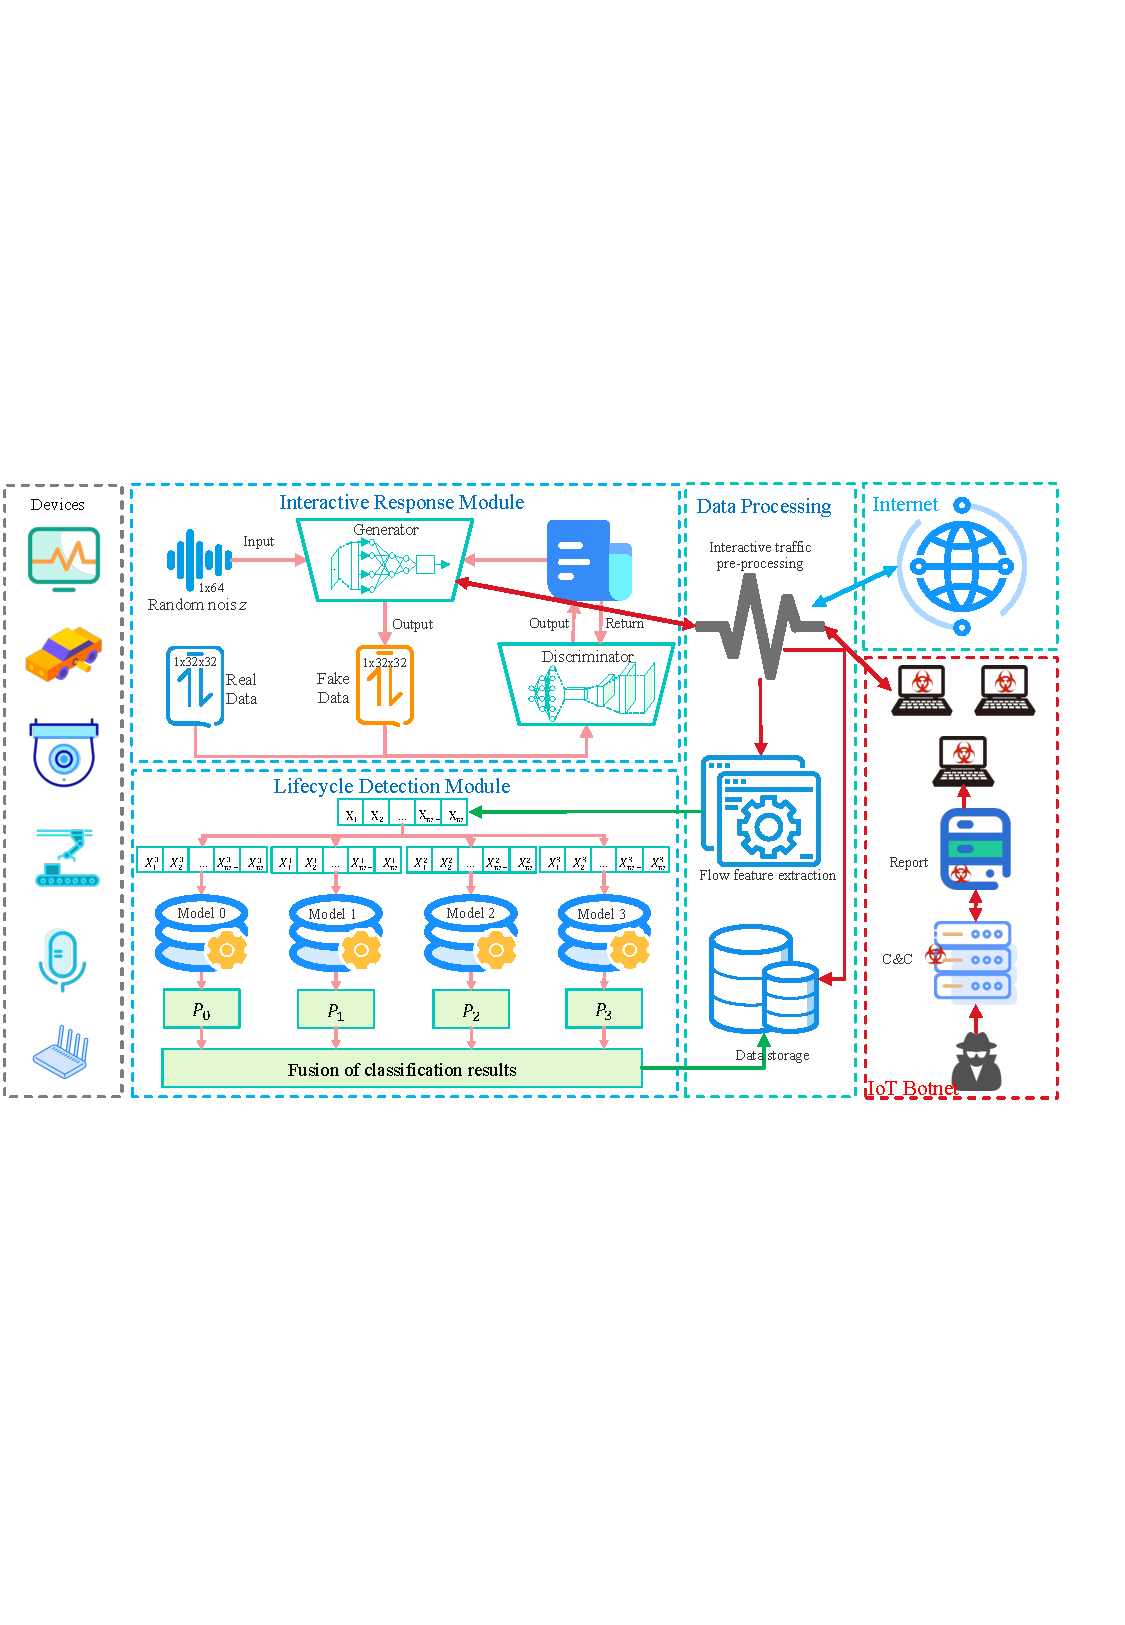
\includegraphics[width = \textwidth]{Figures/structure.pdf}
	\caption{Schematic diagram of the RGPot structure.}
	\label{structure}
\end{figure*}


\section{Proposed Framework}
\label{Proposed Framework}

We present our approach to safeguarding IoT devices from botnet infections through the implementation of a generative model-based honeypot system called RGPot as shown in Figure \ref{structure}. 
RGPot is strategically positioned at the network edge of the IoT environment and is composed of three core components: the data processing module, the interaction response module, and the lifecycle detection module.

\textbf{Data Processing Module: }
This module is responsible for many key functions including interactive traffic processing, traffic feature extraction and data storage.
Interactive traffic processing transforms traffic data into input and output formats suitable for model generation.
Traffic data is stored as pcap files for use in the lifecycle detection process.
Flow feature extraction extracts flow-level features from the pcap data that can be used by the lifecycle detection module for analysis and detection.
Data storage maintains interactive traffic data and classification results.

\textbf{Interaction Response Module: }
The purpose of this module is to use GANs to generate realistic response data based on the received request data.
The generator and discriminator are trained using the dataset.
The converged generative model generates fake data and generates the corresponding response data after inputting the request data into the generator.

\textbf{Lifecycle Detection Module: }
The function of this module is to detect traffic corresponding to specific phases of the IoT botnet lifecycle.
Detection models for each stage of the benign and botnet lifecycle are trained using the dataset.
These trained models are then used to evaluate the input traffic features.
The predictions of each model are fused to produce a final classification of that traffic.

This structured approach, integrating data processing, interaction response, and lifecycle detection modules, forms the foundation of RGPot and contributes to its effectiveness in IoT botnet lifecycle detection and defence.



\subsection{Data Processing Module}
\label{Data processing module}
The data processing module serves several important functions: processing interactive traffic data for the interaction response module, extracting flow features for the lifecycle detection module, and storing both traffic data and detection results. 
This section is dedicated to discussing the critical techniques for implementing interactive flow processing and flow feature extraction.



\subsubsection{Interactive traffic processing}
\label{Interactive traffic processing}

The interaction response module in the GANs predominantly utilizes a convolutional neural network structure. 
To facilitate this process, the response load needs to be encoded in byte format before being converted into an image. 
To achieve this, we propose a byte data bit-level coding algorithm, detailed in Algorithm \ref{coding}.


\begin{algorithm}[!h]
	\small
	\caption{Byte Data Bit Level Coding Algorithm}
	\label{coding}
	\SetKwInOut{Input}{Input}
	\SetKwInOut{Output}{Output}
	
	\Input{Number of bytes encoded per row of the matrix $rN$, Data to be encoded $data$}
	\Output{Coding matrix$matrix$}
	$dataLen = $len($data$);  {\tcp*[h] Get the length of the encoded byte data}\\
	$rowNum = dataLen \times 2$; {\tcp*[h] Get the number of rows in the encoding matrix}\\
	$colNum = rN \times 16$; {\tcp*[h] Get the number of columns in the generated matrix}\\
	$matrix$ = initMatrix($rowNum$, $colNum$); {\tcp*[h]Initialising the coding matrix}\\
	
	\For{$i \leftarrow 1$ \KwTo $dataLen$\\}
	{
		$c = data[i]$;{\tcp*[h] Get the ith byte of the encoded data} 
		$bitArray = $getBitArrayFromByte$(c)$;{\tcp*[h] Get Bit Array}\\
		\For{$j \leftarrow 1$ \KwTo len$(bitArray)$\\}
		{
			$b = bitArray[j]$; {\tcp*[h] Get the value of the $j$ th bit}
			
			$rowStart = i / rN \times 2$;{\tcp*[h] Calculate the starting row of the fill matrix}
			
			$colStart = I / rN \times 16 + j \times 2$; {\tcp*[h] Calculate the starting column of the fill matrix}
			
			{\tcp*[h] Fill the four adjacent elements of the matrix}
			
			$matrix[rowStart][colStart] = b \times 255$;\\
			$matrix[rowStart][colStart + 1] = b \times 255$;\\
			$matrix[rowStart + 1][colStart] = b \times 255$;\\
			$matrix[rowStart + 1][colStart + 1] = b \times 255$;\\
		}
	}
	\Return matrix
\end{algorithm}

The algorithm takes as input the number of encodable bytes per row ($rN$) of the coding matrix and the array of bytes ($data$) to be coded. 
The output of this algorithm is the coding matrix, which can be directly converted into a greyscale map.

The core concept of the algorithm is to map each bit of every byte into four designated elements within the encoding matrix, following a specific order. 
The algorithm operates based on bits as the fundamental unit for populating the matrix.
It scales the bit values by a factor of 255 before incorporating them into the matrix. This scaling enhances the differentiation between elements populated with distinct bit values. 
This approach allows the generator to learn the data distribution at the bit level more effectively and increases the visibility of boundaries between sample values.

Furthermore, the bias-induced predicted values generated by the neural network tend to fall within a proximity range of the true values. 
Within this proximity range, only true values exist, thereby enhancing prediction accuracy. 
Each bit populated into the matrix occupies the position of four neighbouring elements, not just one.
To represent the predicted value of the bit during decoding, the average of these four elements is used.
This practice minimizes prediction errors stemming from generator bias, resulting in more accurate predictions.




The decoding algorithm serves as the reverse process of Algorithm \ref{coding}. 
It works by taking the average of the four neighbouring elements in the coding matrix and comparing it to a predetermined threshold value to determine the predicted bit value.

The byte data bit-level coding algorithm exhibits a time complexity of $O(n^2)$ and a space complexity of $O(n)$. 
This approach offers several advantages, including:
High Information Richness: 
Each element in the resulting matrix encapsulates detailed information from the data being coded at the bit level, ensuring high information richness.
High Information Relevance: 
By presenting information at the bit level, the numerical relevance of the encoded elements is better preserved. This enhances the utility and interpretability of the encoded data.

Overall, the approach not only efficiently encodes data at a fine-grained level but also preserves informational richness and relevance, making it a valuable technique for use in generative models like GANs.











\subsubsection{Flow Feature Extraction}
\label{IoT Botnet Traffic Data Preprocessing}

The data processed by the lifecycle detection module operates at the flow level. 
In the preprocessing of data for classification models, normalization and feature extraction play a pivotal role, as highlighted in previous research\cite{ACARALI20161}.

\textbf{Normalization} is the procedure of rescaling data to fit within the range of $[0, 1]$ through a linear transformation. 
This transformation ensures that the newly scaled data maintains the same order as the original data. 
Normalization is crucial because certain activation functions, such as the Sigmoid and Tanh functions, tend to produce output values that approach constants (0 or 1) for large input values. 
This can lead to the vanishing gradient problem. 
Normalization effectively mitigates this issue by restricting input data within the effective gradient range of these activation functions. 
Additionally, normalization accelerates the convergence speed of the model during training. The normalization function employed in this study is represented in equation \eqref{to_one}:

\begin{align}
		x_{i}^{\prime}=\left(x_{i}-x_{\min }\right) \frac{(b-a)}{\left(x_{\max }-x_{\min }\right)}+a
		\label{to_one}
\end{align}
In the equation, $x_{min}$ represents the numerical minimum value of the same feature, while $x_{max}$ represents the numerical maximum value of that feature. 
Parameters $a$ and $b$ denote the lower and upper bounds of the interval $[a, b]$ to which the original values are scaled. 
The variable $x_i$ signifies the ith numerical value of the same feature, and ${x^{'}}_{i}$ signifies the new eigenvalue achieved after normalization, satisfying the condition ${x^{'}}_{i} \in [a, b]$.

Regarding flow feature extraction, we employed the CICFlowMeter tool \cite{10075591}. 
This tool, developed by Arash, a cybersecurity researcher at New York University, is widely used in cybersecurity datasets for extracting traffic features.

\begin{figure*}[!h]
	\centering
	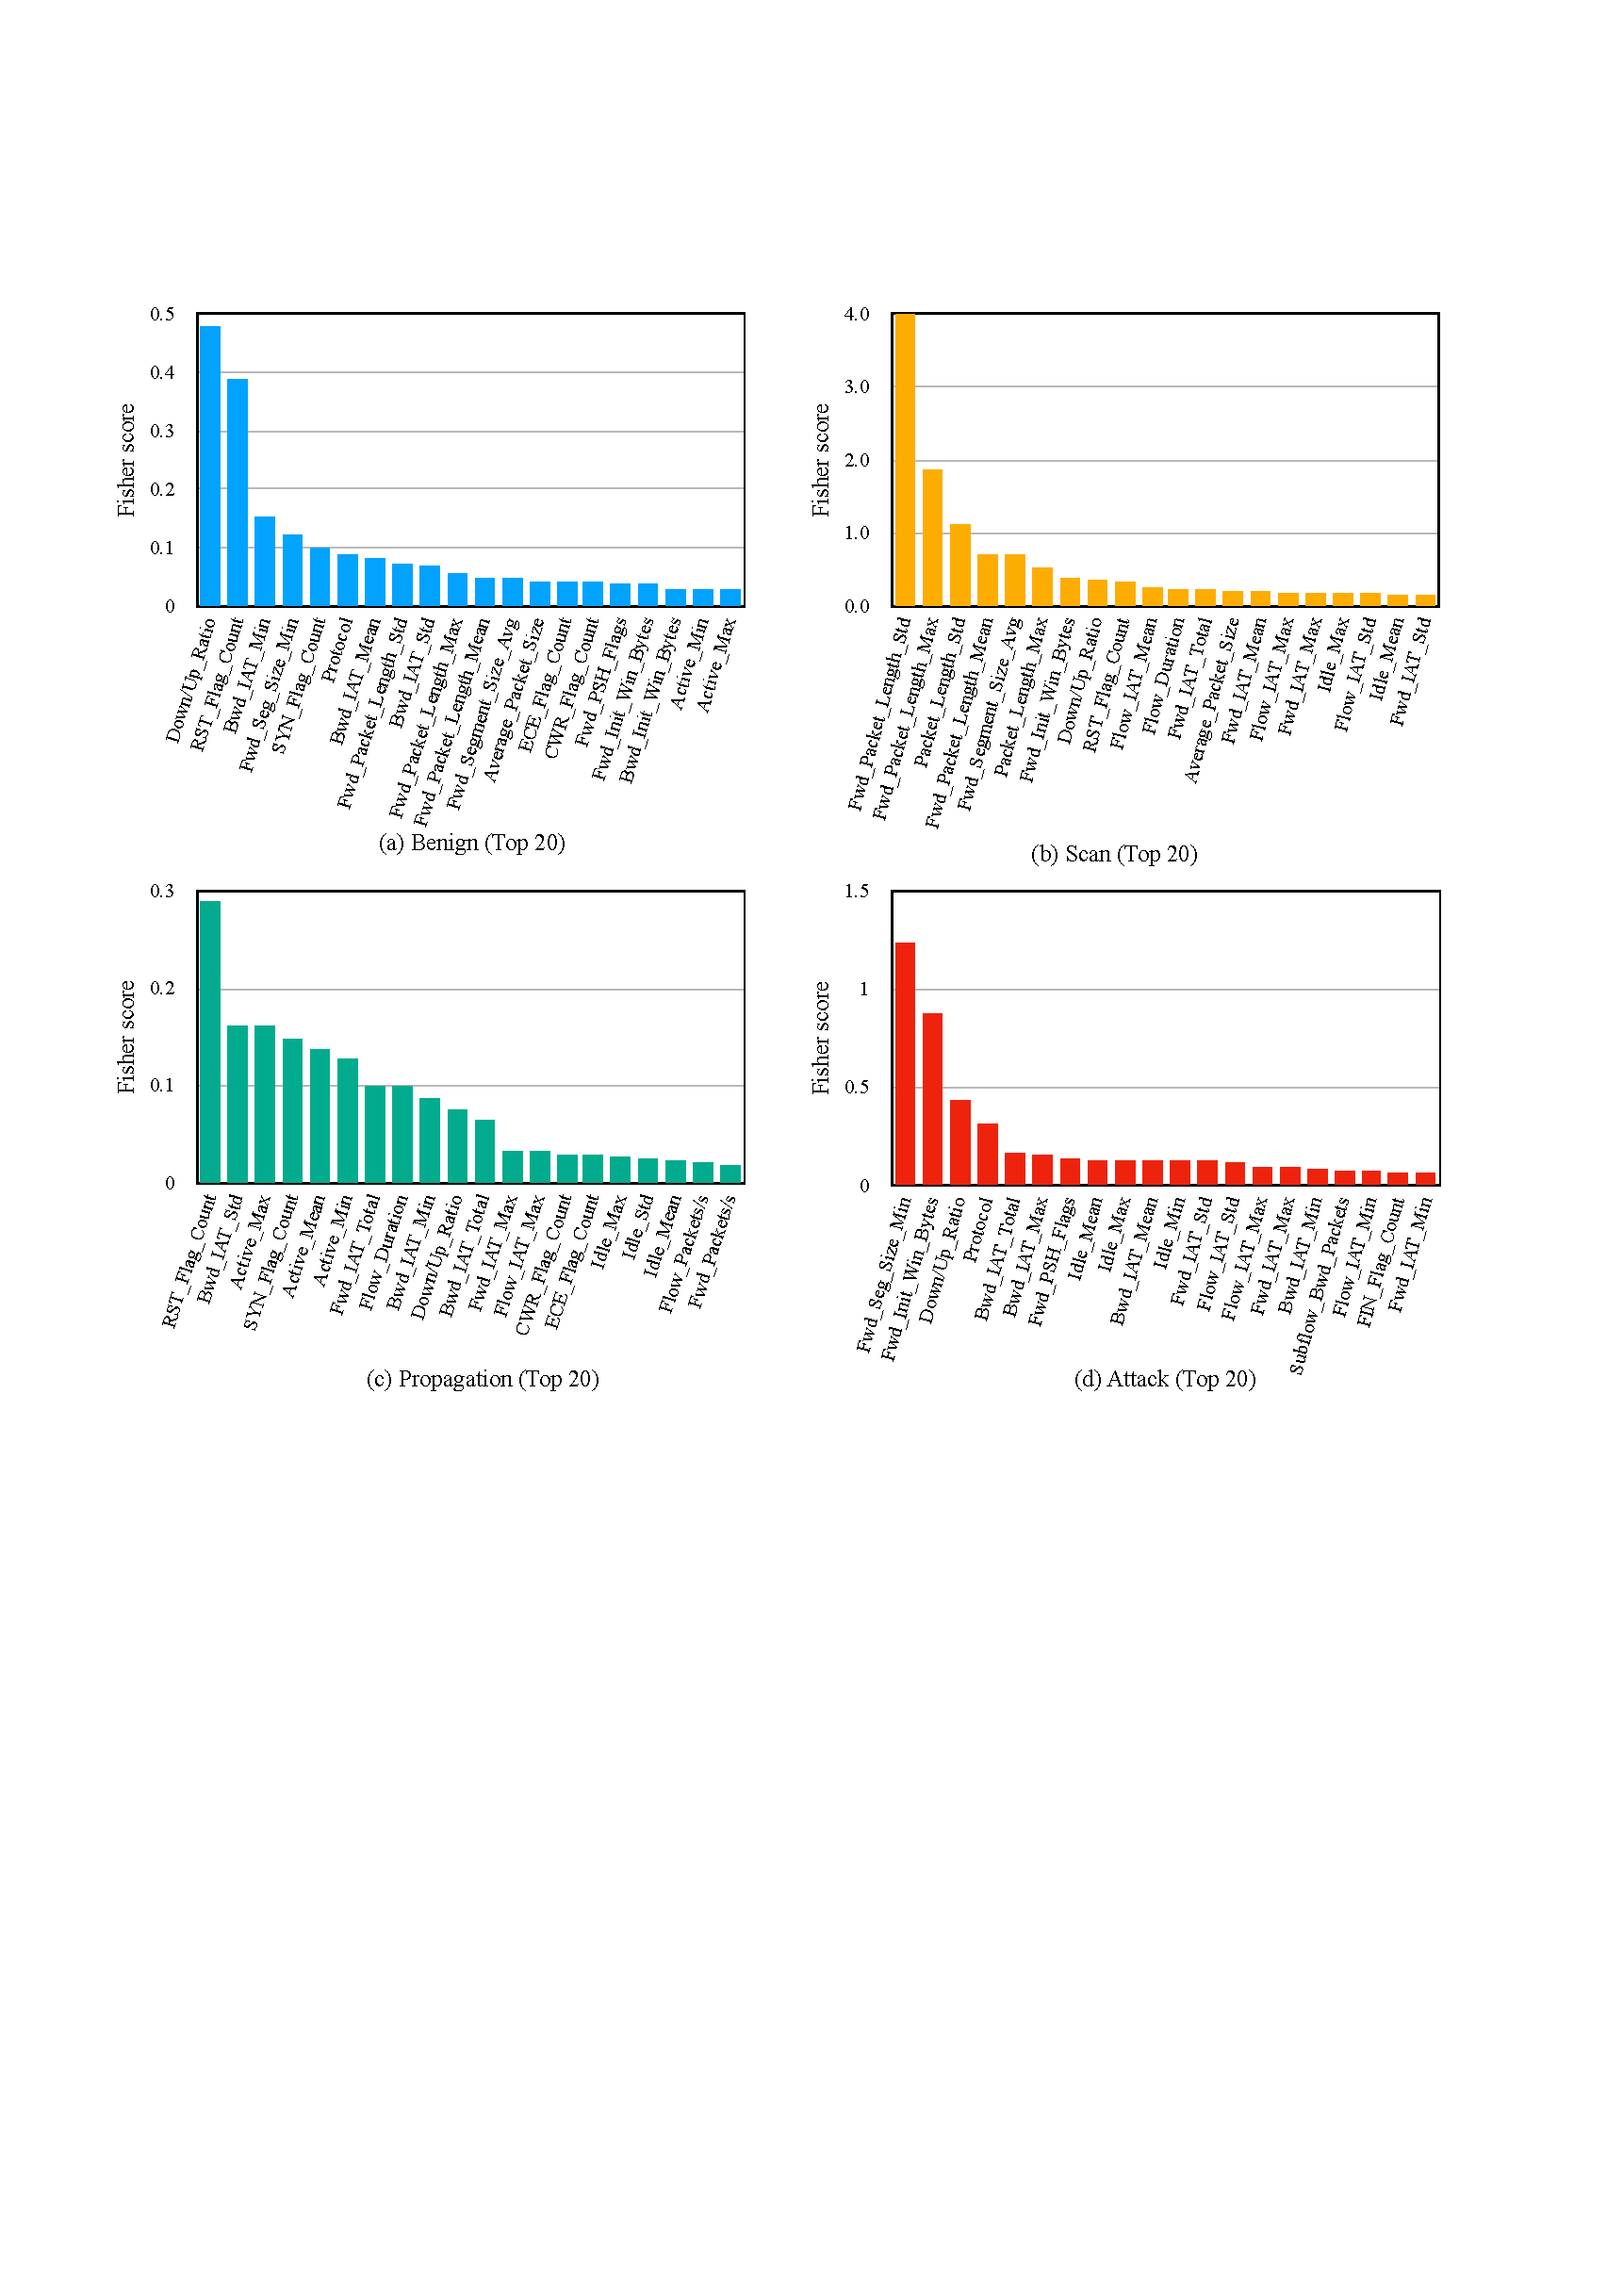
\includegraphics[width = 0.7\linewidth]{Figures/Important_characteristics.pdf}
	\caption{Important characteristics of the various categories of flows (Top 20).}
	\label{Important_characteristics}
\end{figure*}

Given that CICFlowMeter extracts a substantial number of features (approximately 80), the high dimensionality of these features can potentially lead to overfitting and slow down the model convergence during the training process. Moreover, an excessive number of dimensional features can increase computational resource requirements and prolong the time consumed during model detection.



To optimize the feature set for model detection and mitigate these issues, we employed a feature selection approach. 
We ranked the importance of the 80 features extracted by CICFlowMeter using Fisher Score \cite{10075591} and selected the top-ranked features as input features for the classification model.
The Fisher Score is used to identify "good" features that minimize the differences in features between similar classes and maximize the differences between different classes. 
The Fisher Score calculation is depicted in formula \eqref{FisherScore}:

\begin{align}
		F_{s}=\frac{\sum_{j=1}^{K} p_{j}\left(\mu_{j}^{i}-\mu^{i}\right)^{2}}{\sum_{j=1}^{K} p_{j}\left(\sigma_{j}^{i}\right)^{2}}
		\label{FisherScore}
	\end{align}
In the formula, $K$ represents the number of classes; $p_j$ represents the ratio of the total data in the $j$-th category to the total data across all categories; $\mu^{i}{j}$ denotes the numerical mean of the $i$-th feature in the $j$-th category; and $\sigma{j}^{i}$ represents the standard deviation of the $i$-th feature in the $j$-th category.

A larger computed Fisher's score $F_{s}$ indicates a greater ability of the $i$-th feature to distinguish one class from another.



Following the calculation of Fisher Scores for benign traffic and various attack traffic separately, we select the top 20 features with the highest Fisher Scores in each class, as illustrated in Figure \ref{Important_characteristics}, for training the model.







\subsection{Interaction Response Module}
\label{Interaction Response Module}
As shown in Figure \ref{structure}, the basic design of the Interactive Response module is derived from the concept of Generative Adversarial Networks (GANs) \cite{8253599, 9850373}.
GANs are enabled to generate synthetic network traffic and attack models that closely resemble the behaviour of real attackers, thus enhancing the reality of the honeypot.
By fusing simulated attack traffic with actual attack traffic, honeypots become more attractive, thus attracting more attackers and accumulating a large amount of information.
This synthetic data helps security experts gain a deeper understanding of attacker strategies and techniques so they can more effectively counter potential threats.

The generators and discriminators of GANs mainly use the structure of convolutional neural networks, so it is necessary to encode the response loads in byte format to transform them into encoding matrices (images). 
To enable the GANs to better learn the data distribution of the same type of request-response load and take into account the training efficiency of the model, the encoding method designed in this paper will be considered from the following two aspects.
1) Space utilisation: Improving space utilisation is conducive to reducing the size of the coding matrix (image), thus reducing the memory space and other computational resources, and improving the training efficiency of the generative adversarial network; 
2) The degree of information recovery, as far as possible to restore the data distribution of the encoded elements, so that the generator can accurately learn the data distribution on the original data, and as far as possible to mitigate the generator bias caused by the decoding data error when generating samples decoding.



In this paper, the generator receives a single channel with an input dimension of 64 random noise vectors and generates a fake sample with only one channel - a 32$\times$32 greyscale image.
The discriminator receives both the actual sample and the sample generated by the generator and then outputs a probability value between 0 and 1, indicating the possibility that the input is a real sample.
The generator and the discriminator are constantly iterating and competing, gradually enhancing their respective abilities.
Eventually, the two networks reach a dynamic equilibrium where the generator produces samples that appear to the discriminator to be indistinguishable from real samples.
This state is often referred to as convergence.


The generator takes a one-channel, 64-dimensional random noise vector as input, and generates a pseudo-sample in the form of a one-channel grayscale map with a dimension of 32$\times$32. 
The generator is structured as a seven-layer network, designed as follows:

\begin{itemize}
	\item \textbf{Input layer:} The initial layer in the fully connected network comprises 64 neurons and accepts random noise with an input dimension of (64, 1).

    \item \textbf{Hidden layer:} The second layer in the fully connected network consists of 1024 neurons.
    It serves to non-linearly transform the input random noise (64, 1) and conveys the transformed information to the subsequent output layer.

    \item \textbf{Output Layer:} As the final layer in the fully connected network, this layer is composed of 16,384 neurons. 
    It is responsible for producing the information obtained by transforming the input random noise within the fully connected layer, resulting in an output dimension of (16,384, 1).

    \item \textbf{Reshape layer:} The 16,384-dimensional vector, with a single channel, emanating from the fully connected layer, is converted into a feature map with 256 channels and dimensions of (8, 8). 
    This transformation allows the next layer to utilize convolutional algorithms for feature extraction.

    \item \textbf{First Layer Inverse Convolution:} This step employs a convolutional kernel with 64 channels and dimensions of 2$\times$2. It has a stride length of 2 in both horizontal and vertical directions. 
    The role of this layer is to extract features from the feature map and simultaneously reduce the number of channels in the output feature map to 64. 
    This leads to an increase in the dimensions of the feature map to 16x16.

    \item \textbf{Second Layer Inverse Convolution:} Similar to the first layer, this step uses a convolutional kernel with 32 channels, 2$\times$2 dimensions, and a stride length of 2 in both directions. 
    After this layer, the output feature map has 32 channels, with dimensions increased to 32$\times$32.

    \item \textbf{Convolution Layer:} The final layer of the generator employs a convolutional kernel with one channel and 1$\times$1 dimensions. The stride length is both horizontal and vertical. 
    This layer is designed to transform the output of the preceding layers into a matrix with target dimensions, allowing it to be converted into a grayscale map that matches the dimensions of the training samples.


\end{itemize}


The structure of the discriminator primarily consists of a fully connected network. 
The input to this network is a grayscale image with a single channel and dimensions of 32$\times$32. 
The output is a value within the range of (0, 1), where 0 denotes that the input picture is a fake sample, and 1 signifies that the input picture is a genuine sample. 
The discriminator's specific structure is as follows:

\begin{itemize}
    \item \textbf{Reshape Layer:} To feed a grayscale image with one channel and dimensions of 32$\times$32 into a fully connected network, this layer spreads the input grayscale image into a tensor with 1024 channels.

    \item \textbf{Input Layer:} Comprising 1024 neurons, this layer accepts a tensor of dimension (1024, 1) as input and linearly transforms the input data before passing it to the hidden layer.

    \item \textbf{Hidden Layer:} With 512 neurons, this layer introduces a non-linear transformation, enhancing the network's ability to classify complex, nonlinear data.

    \item \textbf{Output Layer:} The output layer's connectivity layer consists of 256 neurons. 
    Given that the discriminator in this study performs binary classification, the output layer produces a single channel. The Sigmoid function maps the output value to the range of (0, 1). 
    The final output from this layer represents the discriminator's confidence level regarding the authenticity of the input sample.
\end{itemize}





\subsection{Lifecycle Detection Module}
\label{Lifecycle Detection Module}

As illustrated in Figure \ref{structure}, the lifecycle detection module comprises a multi-classification detection layer and a fusion layer for combining the detection results. 
The significant features extracted from the data of the currently detected traffic serve as inputs to the multi-classification detection layer. 
The output value range of each category's detection model is $[0, 1]$, and the input features of the current traffic determine the confidence level for that category.

The detection result fusion layer receives the confidence levels from the output of each classification model in the multi-classification detection layer. 
After consolidating the results from each classifier, the final classification result is determined and output.

The multi-classification detection layer utilizes LSTM as a classification model. 
LSTM is particularly well-suited for sequence-based prediction, enabling it to uncover potential relationships between adjacent features within a sequence of features. This study leverages LSTM as the classification model.

The network structure for the classification models 0, 1, 2, and 3 in the lifecycle detection module is identical and is depicted in Figure \ref{classification model}.

\begin{figure}[!h]
	\centering
	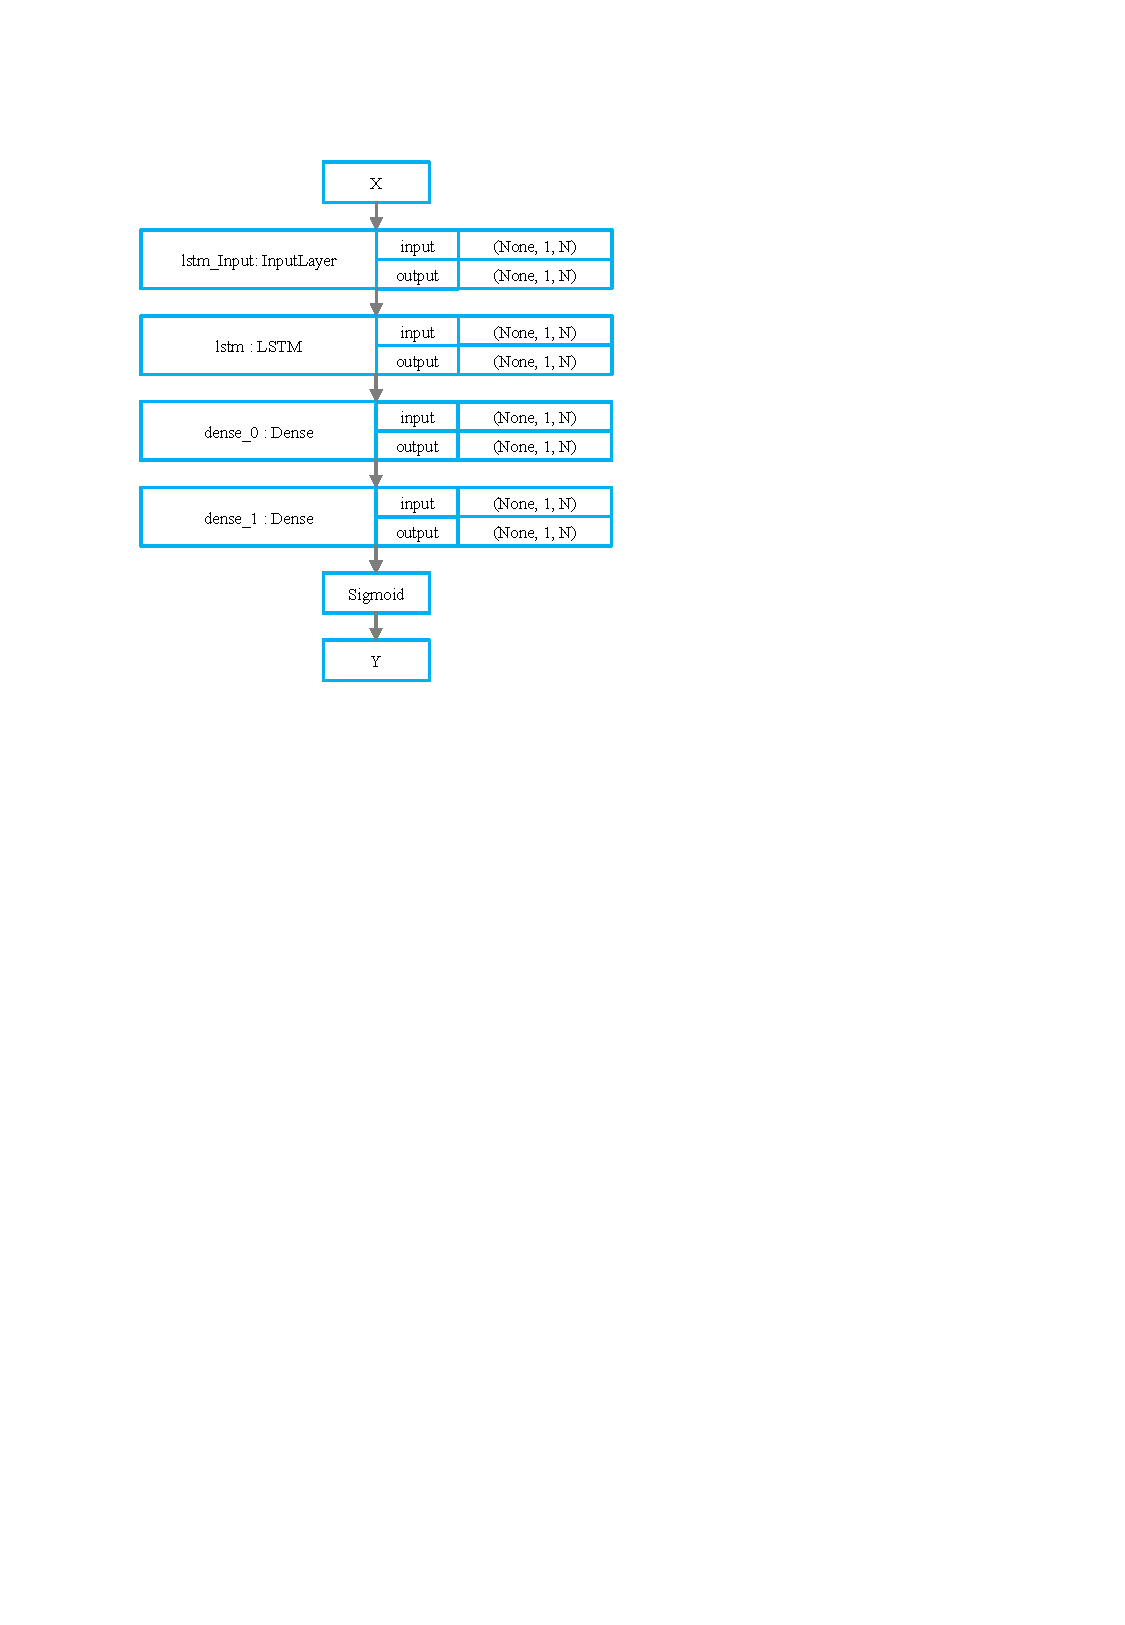
\includegraphics[width = 0.7\linewidth]{Figures/classification model.pdf}
	\caption{Classification model network structure.}
	\label{classification model}
\end{figure}


In Figure \ref{classification model}, the symbol $X$ represents the input feature sequence with a feature dimension of $N$, while $Y$ represents the output prediction result, which falls within the range of $[0, 1]$.

The classification model comprises two primary components. 
The first part is the LSTM layer, which treats the input feature vector of dimension $N$ as a sequence with a length of $N$ and produces an output vector of dimension 10. 
The second part is the fully connected layer. 
The input layer receives a vector of dimension 10 from the LSTM layer and outputs a vector of dimension 40 to the subsequent layer. 
The output layer produces a prediction of dimension 1, which is scaled to the interval $[0, 1]$ using a sigmoid function.

The detection result fusion layer employs a fuser based on a fully connected neural network. 
Initially, the outputs of all classification models in the multi-classification detection layer serve as inputs to the fully connected neural network of the fuser. 
Subsequently, the output of the fully connected neural network's output layer is transformed into the final classification result using the argmax function.

Instead of relying solely on the output of a single classifier, the fuser based on the fully connected neural network combines the outputs of multiple classifiers. 
It updates the connection weights of neurons between adjacent layers in the fully connected neural network through multiple iterations to ensure that the weights of the classification results from multiple classifiers have a more reasonable impact on the final result.

The specific network structure of the fully connected neural network-based fuser in this study is depicted in Figure \ref{fusion layer}. 
It comprises a total of four fully connected layers, with the input and output layers each featuring one fully connected layer, and the hidden layer utilizing two fully connected layers. 
The input layer receives a feature vector of dimension 4, and the output layer produces a feature vector of dimension 4. 
LeakyReLU serves as the activation function between neighbouring fully connected layers.



\begin{figure}[!h]
	\centering
	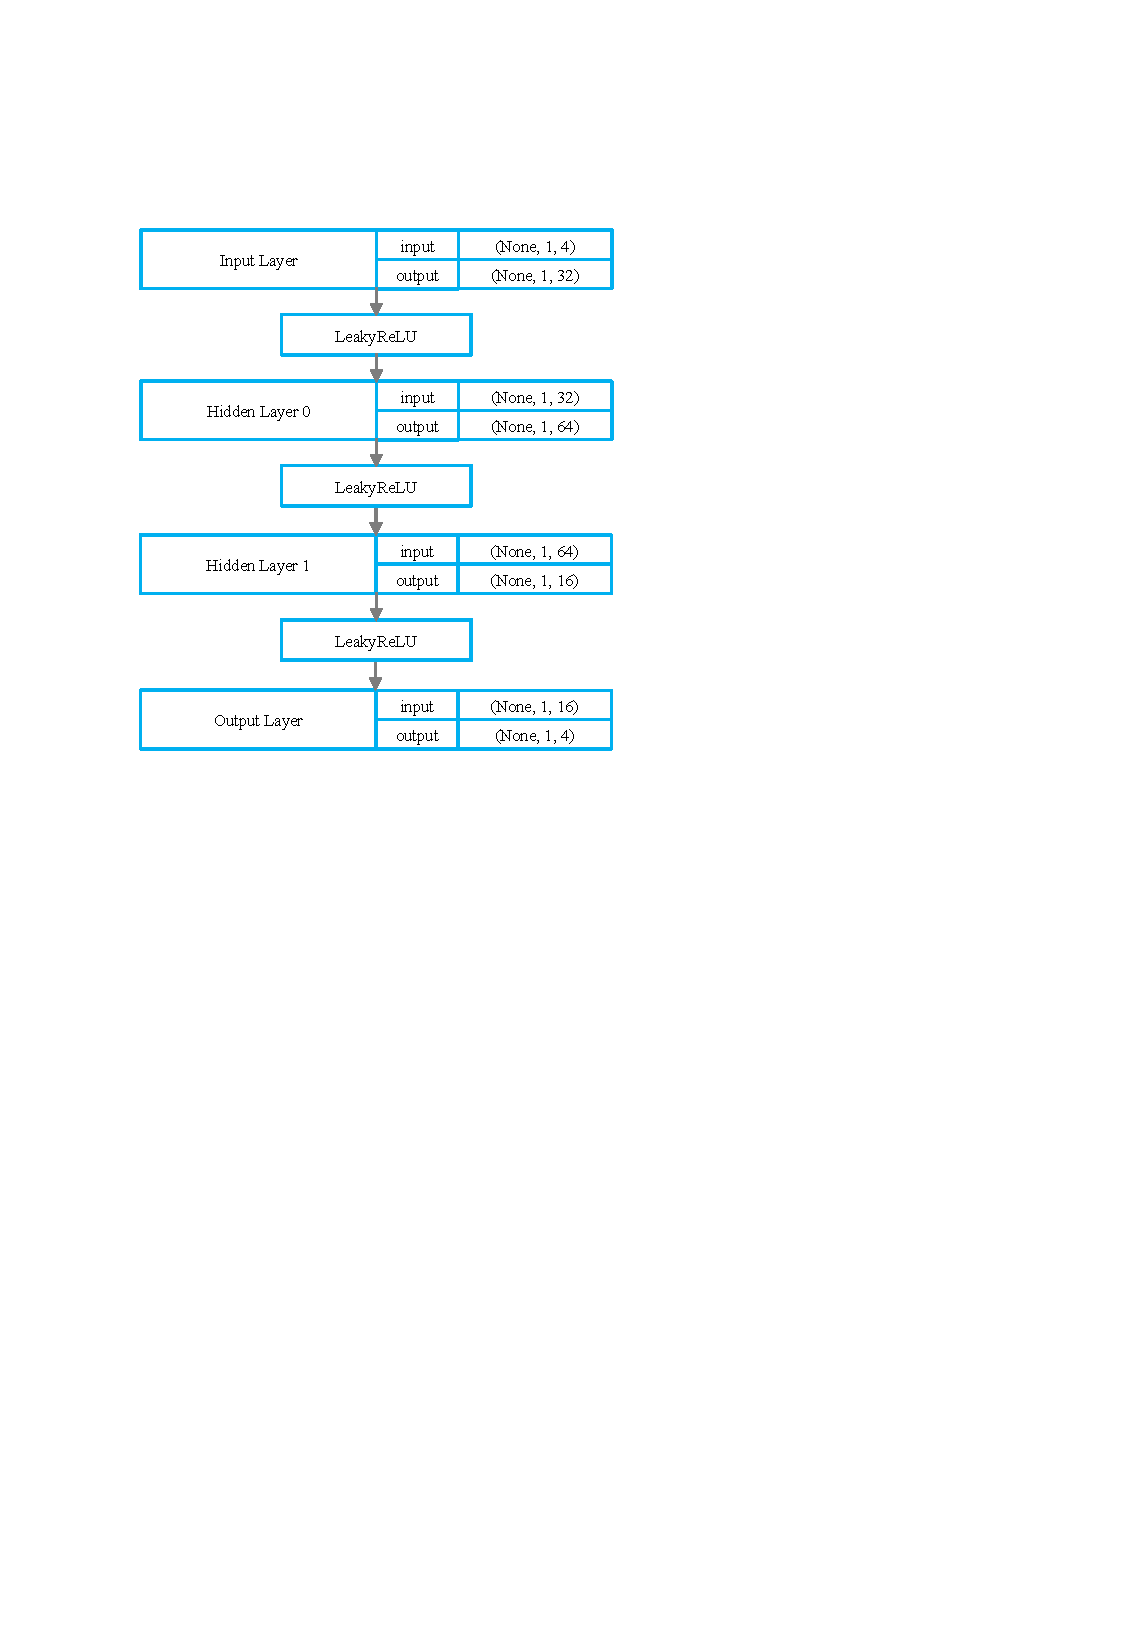
\includegraphics[width = 0.7\linewidth]{Figures/fusion layer.pdf}
	\caption{Classification model network structure.}
	\label{fusion layer}
\end{figure}




\section{Experiments and Analyses}

We first trained the model in RGPot using a training dataset.
Then, we built a simulation experiment environment to test the interaction response module and lifecycle detection module of RGPot and answer the following four key questions:
\begin{itemize}
    \item How realistic is the response data generated by the interaction response module for requests at different phases?
    \item How does RGPot's interaction capability compare to other honeypots?
    \item How effective is the use of fully connected neural networks to fuse results in the lifecycle detection module?
    \item How effective is the detection of IoT lifecycle compared to other classification models?
\end{itemize}



\subsection{Experimental Settings}

\textbf{Experimental Environment Setting:}
In this experiment, we have established a virtual environment using the VMWare platform, where three virtual machines (VMs) are interconnected within the same subnet segment, allowing them to seamlessly communicate through bridge mode. 
Each VM serves a specific purpose in this research setup:

VM1 (Simulated IoT Botnet): Within VM1, we have deployed a simulated IoT botnet. 
This virtual machine emulates the behaviours associated with an IoT botnet, replicating various stages in the botnet's lifecycle, including scanning, propagation, and attack phases.

VM2 (Comparison Service): VM2 runs a comparison service, likely encapsulated within a container. 
This service communicates with the other VMs by using the host's IP address and port, employing the Host network mode. 
VM2 functions as a point of reference for comparative analyses and serves as an integral part of the interactions during the experiment.

VM3 (Netty Server with RGPot): VM3 is equipped with a Netty server running RGPot. 
The Netty server is responsible for exposing the services provided by RGPot through specific ports. 
It can efficiently manage incoming requests, either by extracting application layer data from messages directed to RGPot or by packaging application layer response data for transmission back to the client.

VM1 simulates IoT botnet activities, VM2 provides a baseline for comparison, and VM3 hosts RGPot within a honeypot system, aiming to detect various stages of the IoT botnet lifecycle. 
The orchestrated interactions between these virtual machines are essential for evaluating the effectiveness of RGPot in a controlled environment.

\textbf{Experimental Tasks:}
To validate the performance of RGPot's interaction response module and lifecycle detection module, and to address the research questions (\textbf{Q1} to \textbf{Q4}), four specific experimental tasks have been designed:

\begin{itemize}
    \item Task 1: Effectiveness of data generation at different botnet lifecycle phases.
    This task includes simulating an IoT botnet sending request data with the aim of evaluating the performance of RGPot's data generation capabilities at different phases of the botnet lifecycle.

    \item Task 2: RGPot and Cowrie's ability to interact at different lifecycle phases.
    The focus of Task 2 is to test the ability of RGPot and Cowrie (a well-known honeypot system) to interact at different phases of the IoT botnet lifecycle.
    The aim is to assess how effectively these two systems interact with simulated botnet activity.

    \item Task 3: Convergence analysis of the detection results fusion layer.
    This task aims to analyse the convergence behaviour of the fusion layer responsible for merging the detection results of the lifecycle detection module.
    It will assess how the fusion process improves the overall accuracy and reliability of the classification results.

    \item Task 4: Effectiveness testing of the lifecycle detection module.
    Task 4 focuses on evaluating the effectiveness of the lifecycle detection module and other classification models in identifying the different stages of the IoT botnet lifecycle.
    It evaluates the performance of the module in accurately detecting and classifying botnet activity.

\end{itemize}


These experimental tasks have been thoughtfully designed to comprehensively assess RGPot's capabilities and its effectiveness in detecting various phases of the IoT botnet lifecycle. 
By conducting these tasks, researchers can gain valuable insights into RGPot's performance, providing answers to the research questions and contributing to the field of IoT botnet detection and response.


\textbf{Datasets:}
To train the generative response model and the lifecycle detection model, a training dataset is constructed by combining the MedBIoT and Aposemat IoT-23 datasets. 
This new dataset is designed to ensure a balanced representation of data from different sources.

\begin{itemize}
    \item \textbf{MedBIoT Dataset}: This dataset contains data from three different botnets and captures network traffic from four distinct device types, making it a medium-sized dataset.

    \item \textbf{Aposemat IoT-23 Dataset}: Aposemat IoT-23 is a dataset that includes data from ten botnet types and captures network traffic from four different device types. 
    It is considered a small dataset.
\end{itemize}

By combining these datasets, we aim to create a new, balanced dataset that retains pcap data from ten botnet types and seven different device types.
This new dataset is called “ Mini-dataset".
It is this Mini-dataset that is used to train the Generative Response Model and the Lifecycle Detection Model.
The process of combining these datasets helps to ensure that the generated training dataset is representative of a wide range of botnet and device characteristics.

\textbf{Evaluation Metrics:}
To evaluate the performance of IoT botnet lifecycle detection, we employ several key evaluation metrics, including Accuracy, Precision, Recall, and F1-score. 
Since this is a multi-classification task, we apply weighted evaluation metrics and calculate their average values. 
The definitions of these evaluation metrics are as follows:
True Positive (TP); True Negative (TN); False Positive (FP); False Negative (FN).

The evaluation metrics are calculated as follows:

\textbf{Accuracy:} Accuracy measures the proportion of samples correctly classified by the model. 
It is calculated as the number of samples correctly categorized divided by the total number of samples. 
The formula for accuracy is as follows:
\begin{align}
\small
	\begin{split}
		Accuracy=\frac{1}{N} \sum_{i=1}^{N}\left(f\left(x_{i}\right)==y_{i}\right) 
	\end{split}
	\label{Accuracy}
\end{align}

Accuracy provides an overall assessment of the model's performance, indicating how many samples were correctly classified across all classes.

Next, we have Precision, Recall, and F1-score, which are metrics often used in multi-class classification tasks:

\textbf{Precision:} Precision, also known as Positive Predictive Value, quantifies how many of the positive predictions made by the model are actually correct. It is computed as:
\begin{align}
\small
	\begin{split}
		Precision =\frac{1}{m} \sum_{i=1}^{m} w_{i} \times \frac{T P_{i}}{T P_{i}+F P_{i}} 
	\end{split}
	\label{WeightedP}
\end{align}

A high precision score indicates that when the model predicts a sample as positive, it is often correct.

\textbf{Recall:} Recall, also known as Sensitivity or True Positive Rate, measures the proportion of actual positive samples that are correctly predicted by the model. 
It is calculated as:
\begin{align}
\small
	\begin{split}
		Recall  =\frac{1}{m} \sum_{i=1}^{m} w_{i} \times \frac{T P_{i}}{T P_{i}+F N_{i}} 
	\end{split}
	\label{WeightedR}
\end{align}

A high recall score means the model correctly identifies most of the actual positive samples.

\textbf{F1-score: }The F1-score is the harmonic mean of precision and recall. 
It provides a balance between these two metrics and is especially useful when there is an uneven class distribution. 
The F1-score is calculated as:
\begin{align}
\small
	\begin{split}
	   F1-score = 2 \times \frac{ Precision * Recall}{ Precision+ Recall}
	\end{split}
	\label{WeightedF1}
\end{align}

This metric combines precision and recall, giving equal importance to false positives and false negatives. 
It is a useful measure of a model's overall performance.

These metrics are valuable tools for assessing the effectiveness of an IoT botnet lifecycle detection model, particularly in cases with multiple classes or categories.



In the formulas from \eqref{Accuracy} to \eqref{WeightedF1}, the symbols are defined as follows:
$N$ represents the total number of samples classified.
$f(x_i)$ represents the predicted classification result.
$y_i$ represents the true classification result.
$m$ represents the total number of categories in the multiclassification.
$TP_i$ represents the total number of true instances of the $i$th category in the classification result.
$FP_i$ represents the total number of false positive examples for the $i$th category in the classification result.
$w_i$ represents the weight of the category. In this experiment, $w_i$ represents the proportion of samples in the $i$th category in the test set.
$FN_i$ represents the total number of false negative cases for the $i$th category in the classification result.




\textbf{Comparison Methods:}
To evaluate RGPot's interaction performance, we conducted a comparative analysis with Cowrie\cite{9633881} and designed specific experiments for this purpose.

Cowrie is considered a medium-high interaction honeypot with relatively robust interaction capabilities among IoT honeypots. 
The Cowrie project remains active, receiving continuous updates and improvements to address evolving attack trends and emerging threats.

To validate the classification capabilities of the IoT botnet lifecycle detection model, we designed comparative experiments to assess the proposed method against three general-purpose classification models. 
These models include K-Nearest Neighbors (KNN)\cite{knn}, Support Vector Machine (SVM)\cite{PONMALAR2022108295}, and Long Short-Term Memory (LSTM)\cite{LINDEMANN2021103498}. 
These three algorithms are commonly utilized in the fields of machine learning and deep learning, and they have found widespread application in IoT botnet detection efforts.





\subsection{Performance Comparison and Analysis}
\label{Performance Comparison and Analysis}


In our pursuit to address the four key questions (Q1 to Q4), we meticulously conducted a series of experiments and diligently scrutinized the accompanying results.

\textbf{Result 1: RGPot's Response to Various IoT Communication Protocols (Answering Q1)}

To tackle Q1, we meticulously deployed our innovative RGPot alongside an open-source IoT botnet in a networked environment. This arrangement allowed for interactions between the simulated botnet and RGPot. 
During this experiment, we deliberately emulated protocols that are frequently utilized in IoT communication, including MQTT, CoAP, HTTP, SSH, and Telnet, among others.

For instance, let's delve into the interaction process with Telnet as a representative example, where the simulated infection process of the IoT botnet unfolds as follows:

\begin{itemize}
    \item Connection: The IoT botnet initiates a connection with the device's Telnet service, resulting in the generation of a Telnet Negotiation Options message. 
    This message serves to negotiate Telnet's functional parameters, such as the activation of the display back, window size settings, and more, with the Telnet server on the device.

    \item Brute Force: The IoT botnet engages in a forceful attempt to breach the username and password of the Telnet service on the device. In this particular experiment, 'root' is the chosen username, granting superuser privileges. 
    Subsequently, a password is randomly selected from a dictionary of common passwords (comprising 20 entries) for the brute-force attack.

    \item Malware Deployment: Upon successful login, the IoT botnet proceeds to load malware onto the device via the Echo command and subsequently executes this malicious software.

    \item Heartbeat: The IoT botnet maintains a heartbeat connection with the device through the running malware, enabling the collection of information about uninfected devices from the responses during the heartbeat phase.

\end{itemize}

Figures \ref{Real_Data} and \ref{Fake_Data} depict the real and generated samples corresponding to each interaction stage using grayscale graphs. Each graph signifies a sample from a different phase, encompassing the (a) consultation phase, (b) login verification phase, (c) malware loading phase, (d) malware execution phase, (e) heartbeat hold phase, and (f) message reporting phase.

Upon comparing these two sets of images, it becomes apparent that the data in each encoding position remains distinguishable. 
Nonetheless, there is a discernible difference in grayscale between the two sets of images. 
This observation underscores the encoding accuracy maintained by RGPot in generating grayscale diagrams.




\begin{figure}[!h]
	\centering
	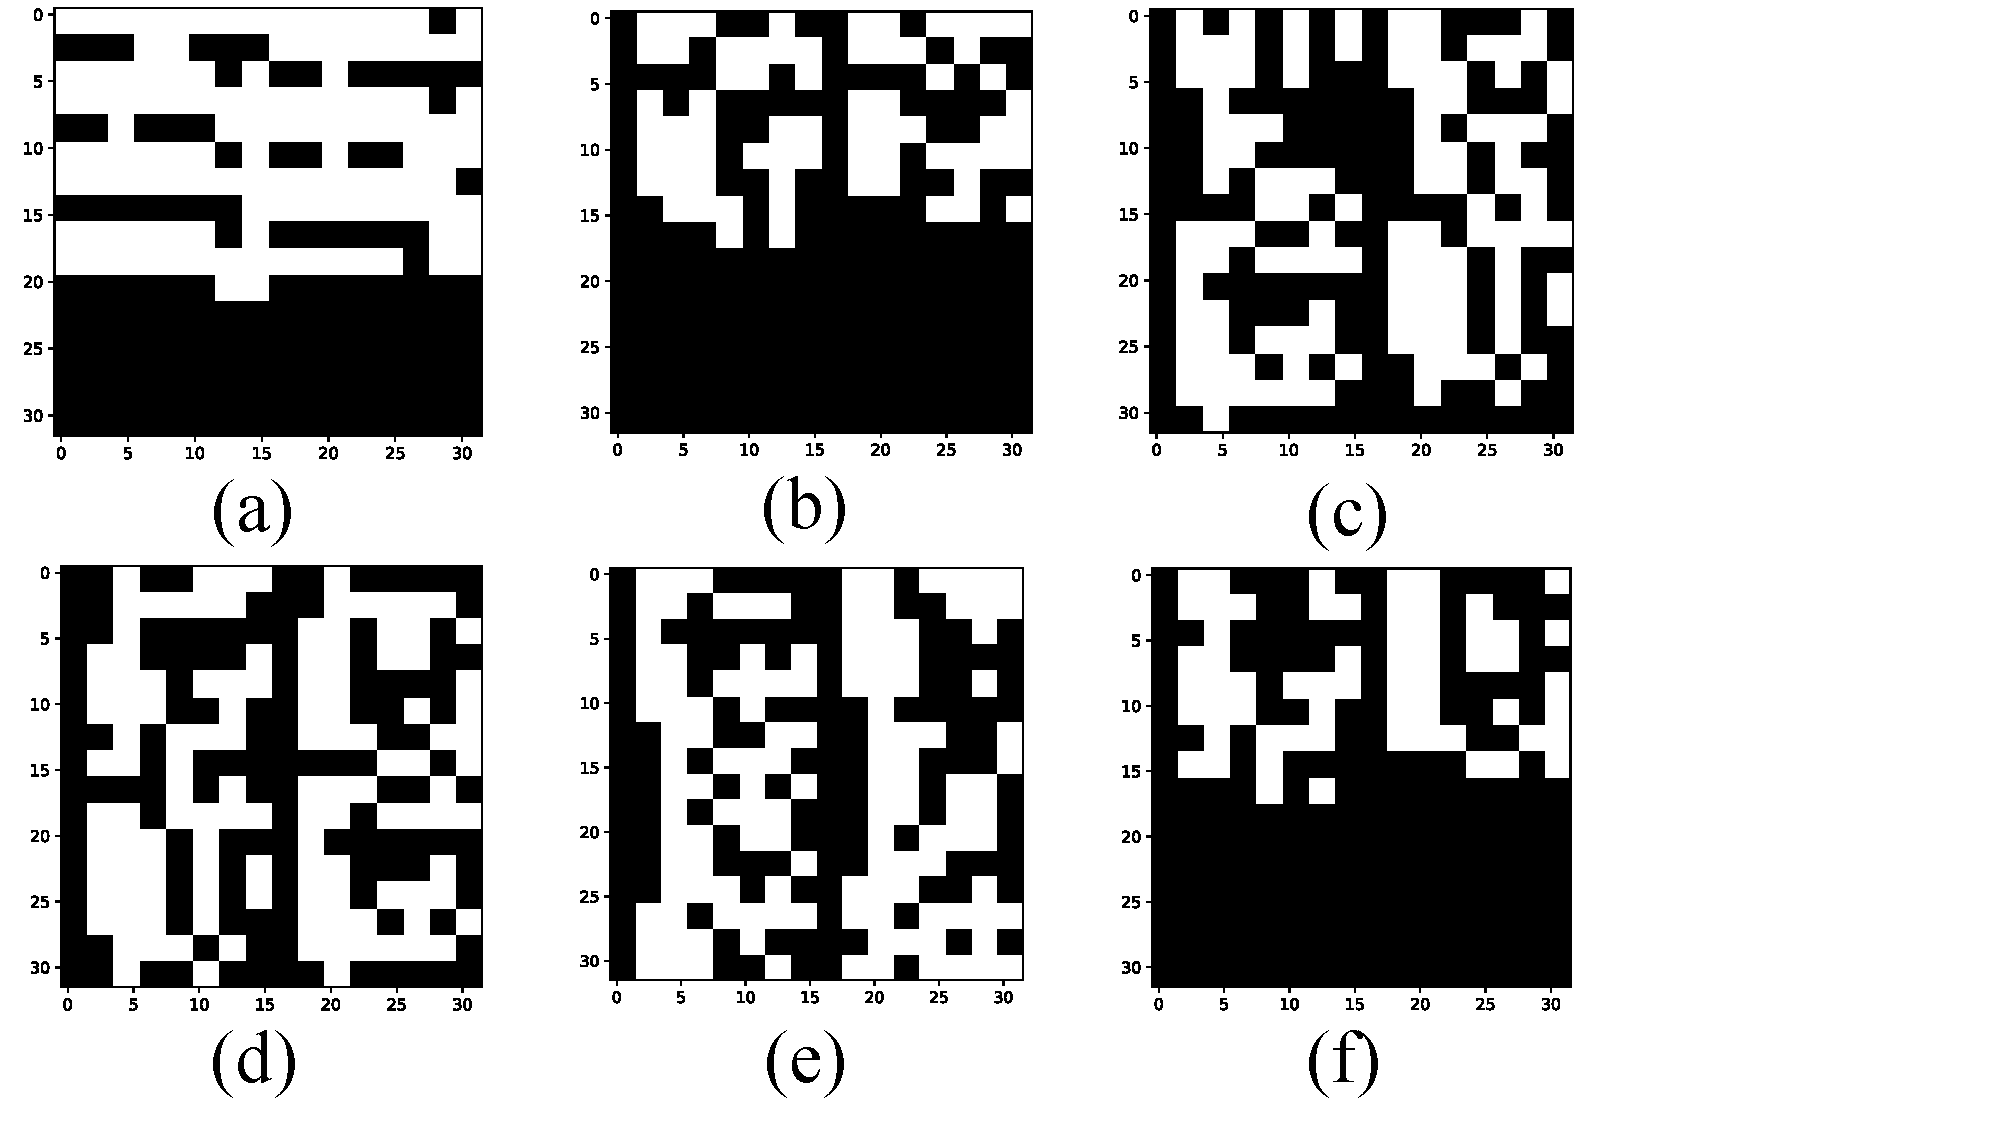
\includegraphics[width = 0.7\linewidth]{Figures/Real_Data.pdf}
	\caption{Real sample coding charts.}
	\label{Real_Data}
\end{figure}

\begin{figure}[!h]
	\centering
	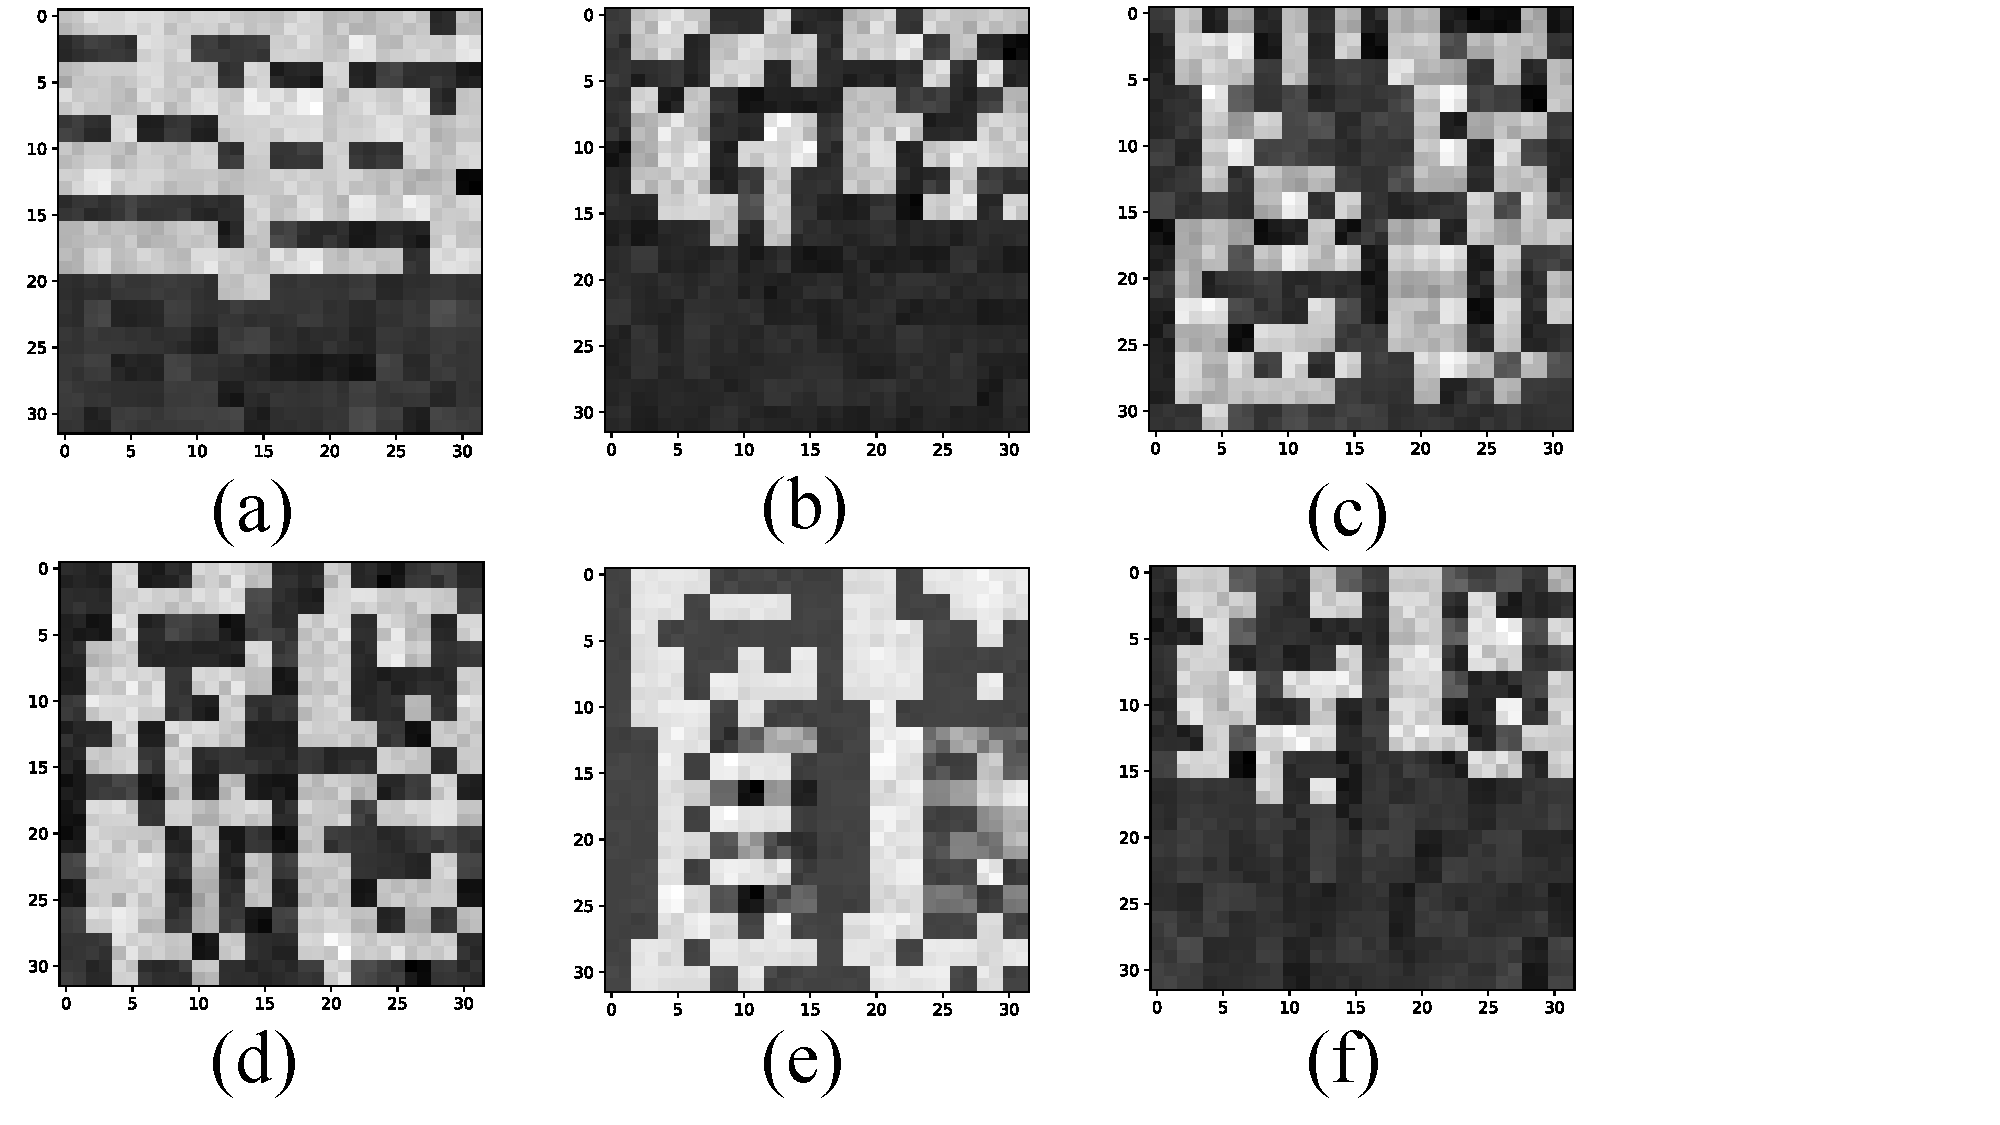
\includegraphics[width = 0.7\linewidth]{Figures/Fake_Data.pdf}
	\caption{Generate sample coding charts.}
	\label{Fake_Data}
\end{figure}

Furthermore, we meticulously conducted 100 tests on the grayscale diagram data from each stage of interaction. 
Table \ref{table3} shows the training of the generator at different interaction stages, where the generation sample correctness is the proportion of generated samples (grey-scale images) that are decoded and transformed to yield a response body (byte-type data) that matches the true response body format.
This high accuracy is attributed to the uniqueness of responses corresponding to each type of request in these phases.

\begin{figure*}[!h]
	\centering
	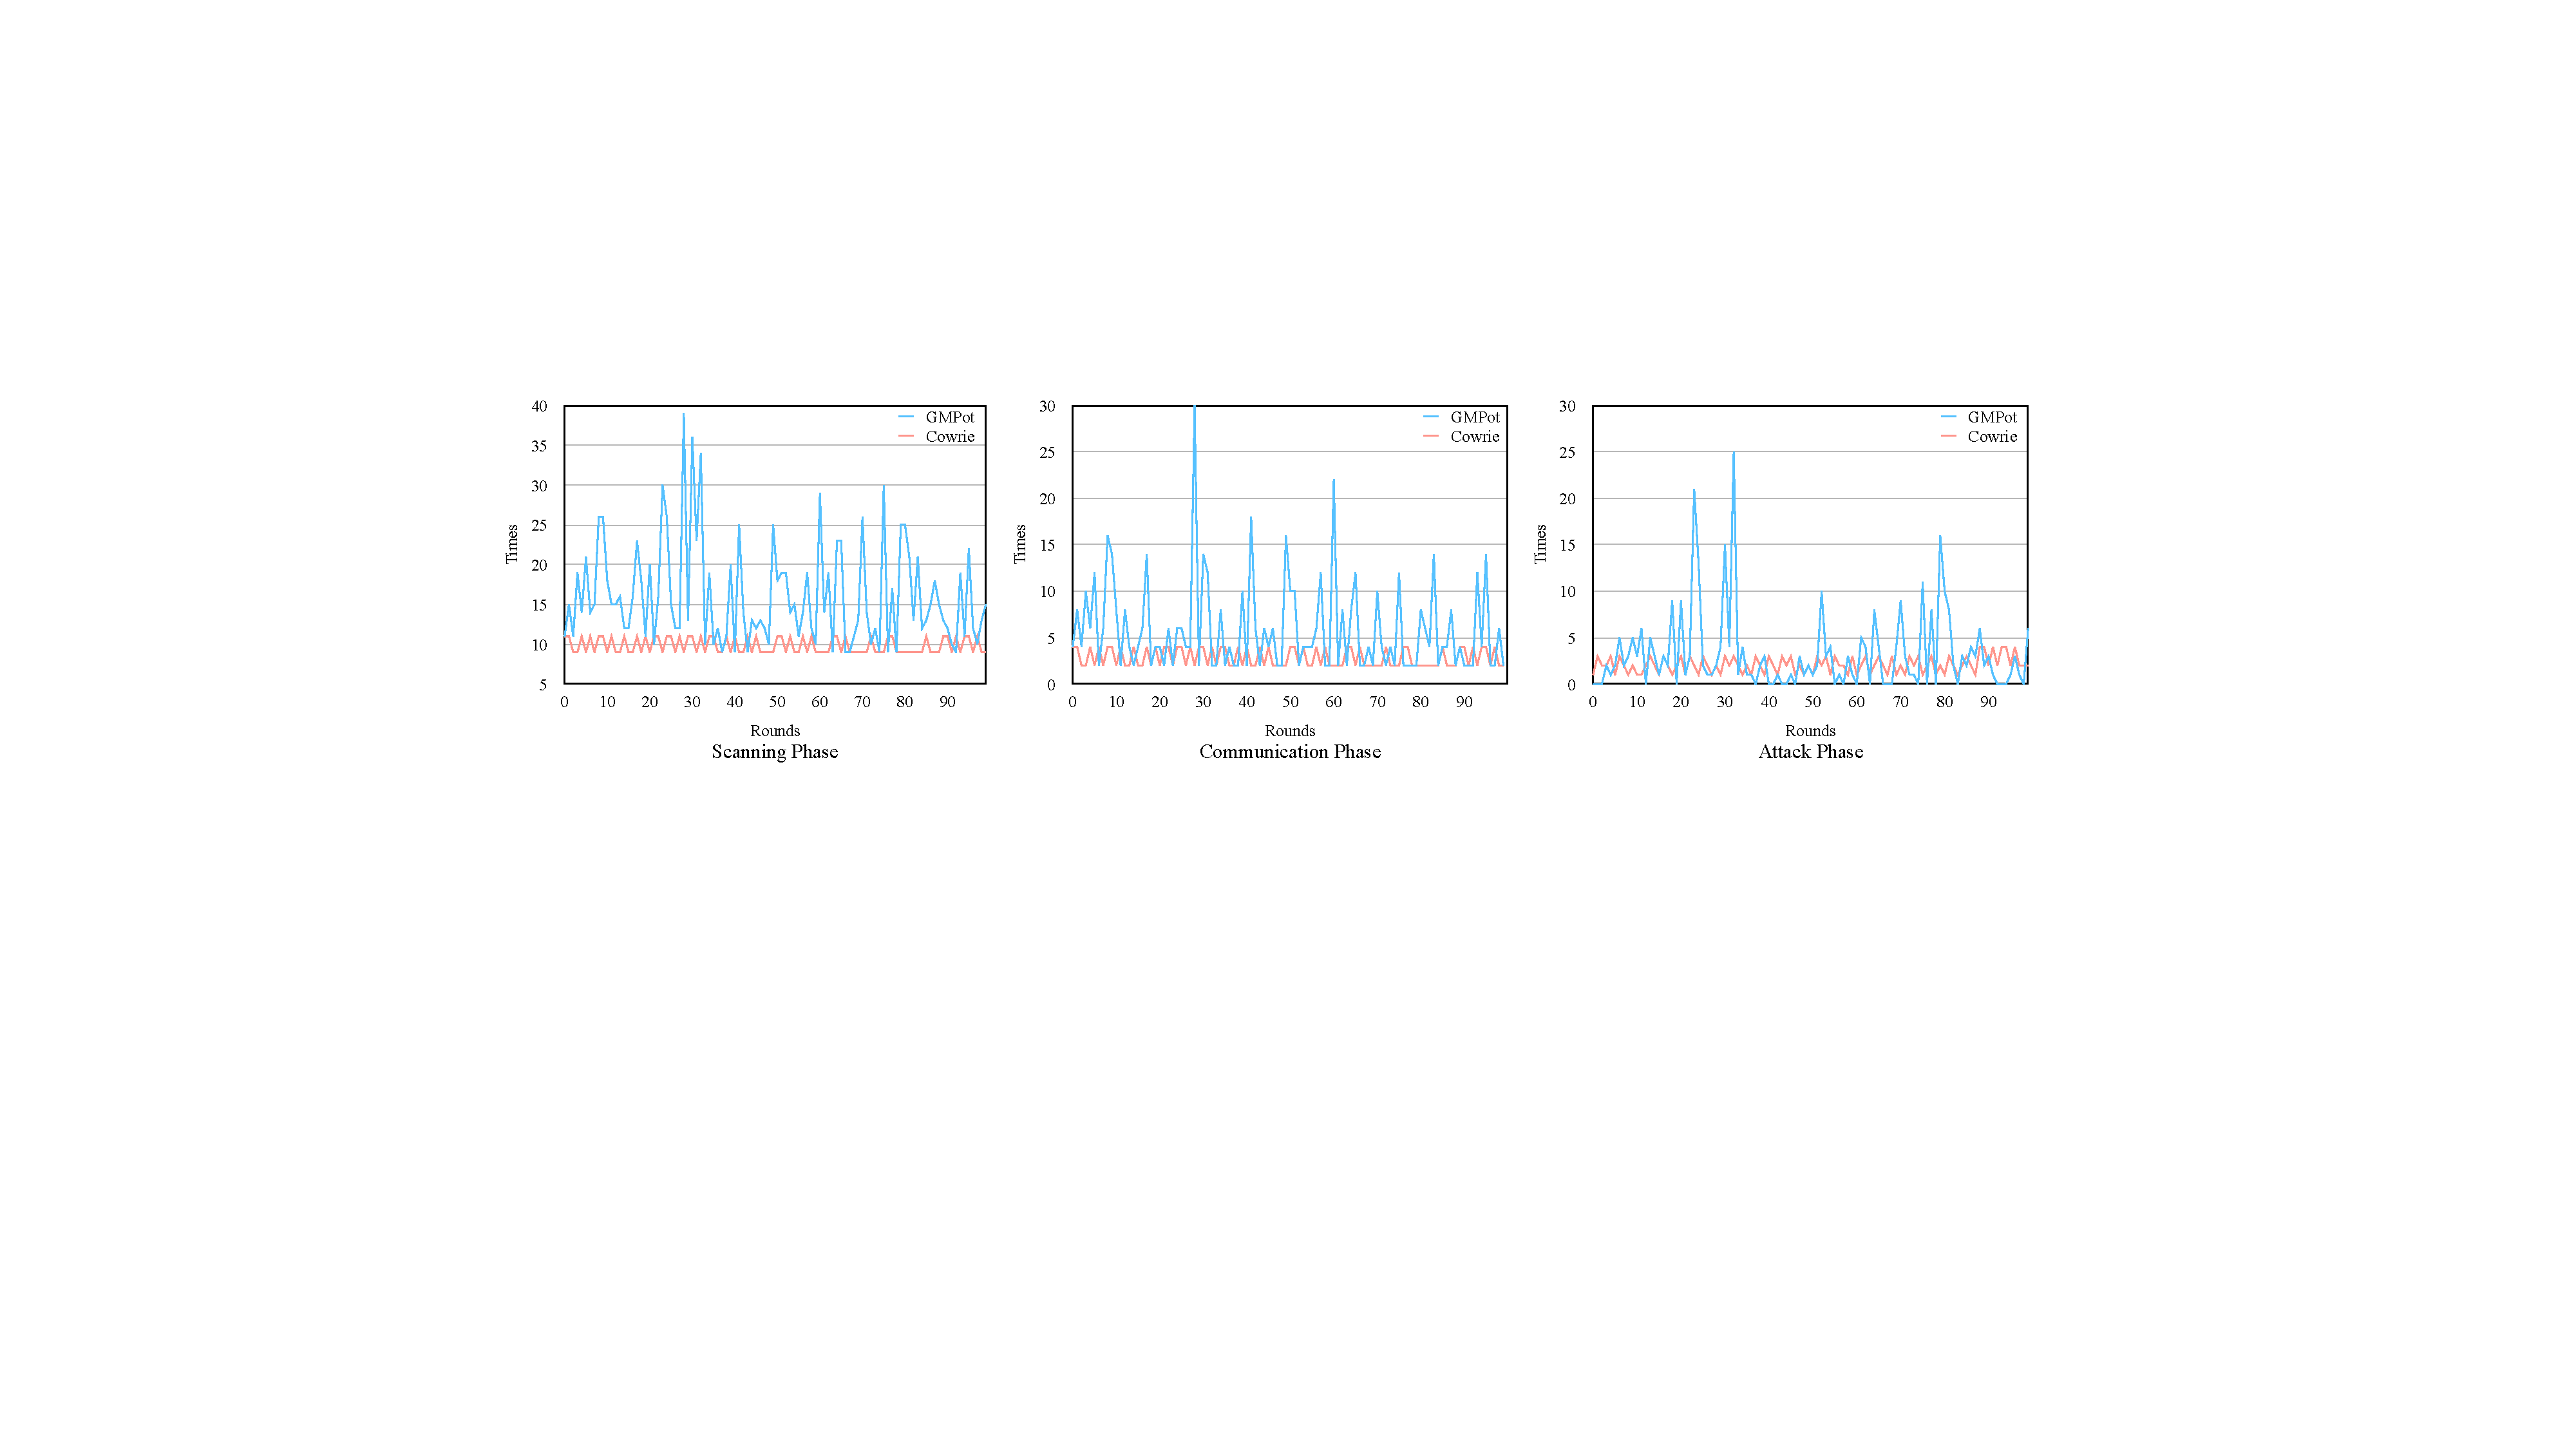
\includegraphics[width = \linewidth]{Figures/Interaction testing at all stages.pdf}
	\caption{Comparison of the number of RGPot and Cowrie interactions.}
	\label{Comparison_of_Interaction_Capabilities}
\end{figure*}

However, in the heartbeat phase, the accuracy of the generated samples is relatively lower due to the presence of a significant variable component in the response packets for this phase. 
Achieving higher accuracy in the generated samples for the heartbeat phase would necessitate additional resource consumption during training.

In aggregate, the overall accuracy rate of the generated samples impressively reaches 94.5\%, signifying the effectiveness and precision of RGPot's sample generation across various phases of interaction.


\begin{table}[!h]
\centering
\caption{Accuracy of sample generation.}
\label{table3}
\begin{tabular}{|cc|c|}
\hline
\multicolumn{1}{|c|}{Sequence} & Interaction Stage           & Accuracy \\ \hline
\multicolumn{1}{|c|}{(a)}      & Option negotiation phase    & 100\%    \\ \hline
\multicolumn{1}{|c|}{(b)}      & Login Verification Phase    & 99\%     \\ \hline
\multicolumn{1}{|c|}{(c)}      & Malware loading phase       & 99\%     \\ \hline
\multicolumn{1}{|c|}{(d)}      & Malware Execution Stage     & 98\%     \\ \hline
\multicolumn{1}{|c|}{(e)}      & Heartbeat Hold              & 76\%     \\ \hline
\multicolumn{1}{|c|}{(f)}      & Information Reporting Phase & 95\%     \\ \hline
\multicolumn{2}{|c|}{All Phase}                              & 94.5\%   \\ \hline
\end{tabular}
\end{table}



Applying the same approach, we conducted training on four additional protocols frequently used in IoT communication: MQTT, CoAp, HTTP, and SSH. The comprehensive results, which also include the Telnet protocol, are thoughtfully presented in Table \ref{table4}. 
This table provides valuable insights into the accuracy of the samples generated for each of these protocols, demonstrating the versatility of RGPot in handling a range of communication methods commonly found in IoT environments.

\begin{table}[!h]
\centering
\caption{Accuracy of samples generated by different protocols.}
\label{table4}
\begin{tabular}{|c|c|c|c|c|c|}
\hline
Protocols & MQTT   & CoAP   & HTTP   & SSH    & Telnet \\ \hline
Accuracy  & 93.3\% & 94.7\% & 96.7\% & 96.1\% & 95.6\% \\ \hline
\end{tabular}
\end{table}




\textbf{Summary:}
Following our experiments, we have confirmed that RGPot consistently achieves an impressive accuracy rate of over 93\% when generating response data in response to various IoT communication protocol request data. 
This remarkable performance can be attributed to the utilization of a generative adversarial network model within the design of RGPot's interaction response module. 
The trained generator excels in producing deceptive responses tailored to different request data, enabling the high level of accuracy observed.





\textbf{Result 2: Comparing Honeypot Interaction Capabilities (Answering Q2)}

To address \textbf{Q2}, this experiment involves a comparison between RGPot and Cowrie, a widely employed open-source honeypot recognized for its medium to high interaction capabilities, using the Telnet protocol as the testing protocol. 
The number of interactions between the honeypot and the IoT botnet is utilized as a simulated metric for evaluating the honeypot's performance.

The primary participants in this experiment are as follows:

1. A simplified Mirai botnet\cite{20195007827865} was employed. 
This simplified version of the Mirai botnet, based on the Telnet protocol, was used to facilitate a direct comparison of interaction levels between the two honeypots. 
It also eliminates the need for duplicative and intricate operations present in the full Mirai infection process.

2. Cowrie, a medium-to-high interaction honeypot, was selected as the reference for comparison.

3. RGPot, the honeypot under evaluation, is the focus of this study..


After conducting 100 rounds of interaction tests, the results regarding the number of interactions per round between RGPot and Cowrie are depicted in Figure \ref{Comparison_of_Interaction_Capabilities}.

The figure clearly illustrates that RGPot consistently outperforms Cowrie in terms of the number of interactions at all stages. Statistically, RGPot achieved an average of 16 interactions per round, with a maximum of 42 interactions. 
In contrast, Cowrie averaged only 5 interactions per round, with a maximum of 11 interactions. 
This means that RGPot had, on average, approximately three times as many interactions as Cowrie, and in one particular round, RGPot achieved a remarkable 42 interactions, which is roughly four times the maximum number of interactions recorded for Cowrie.

\textbf{Summary:}
Based on the experimental tests and theoretical analyses, the comparison between RGPot and Cowrie indicates that RGPot surpasses Cowrie in terms of interaction capabilities. 
This suggests that the response generation module, which relies on generative models within RGPot, can consistently interact with attackers effectively, capturing their attack data.

\textbf{Result 3: Convergence Analysis of Detection Result Fusion (Answering Q3)}



To address Q3, a fully connected neural network-based fuser was trained in the detection result fusion layer. 
After each round of training, the threat perception model was tested using a test set, and the model's classification effect on the test set was recorded for each round.

\begin{figure*}[!h]
	\centering
	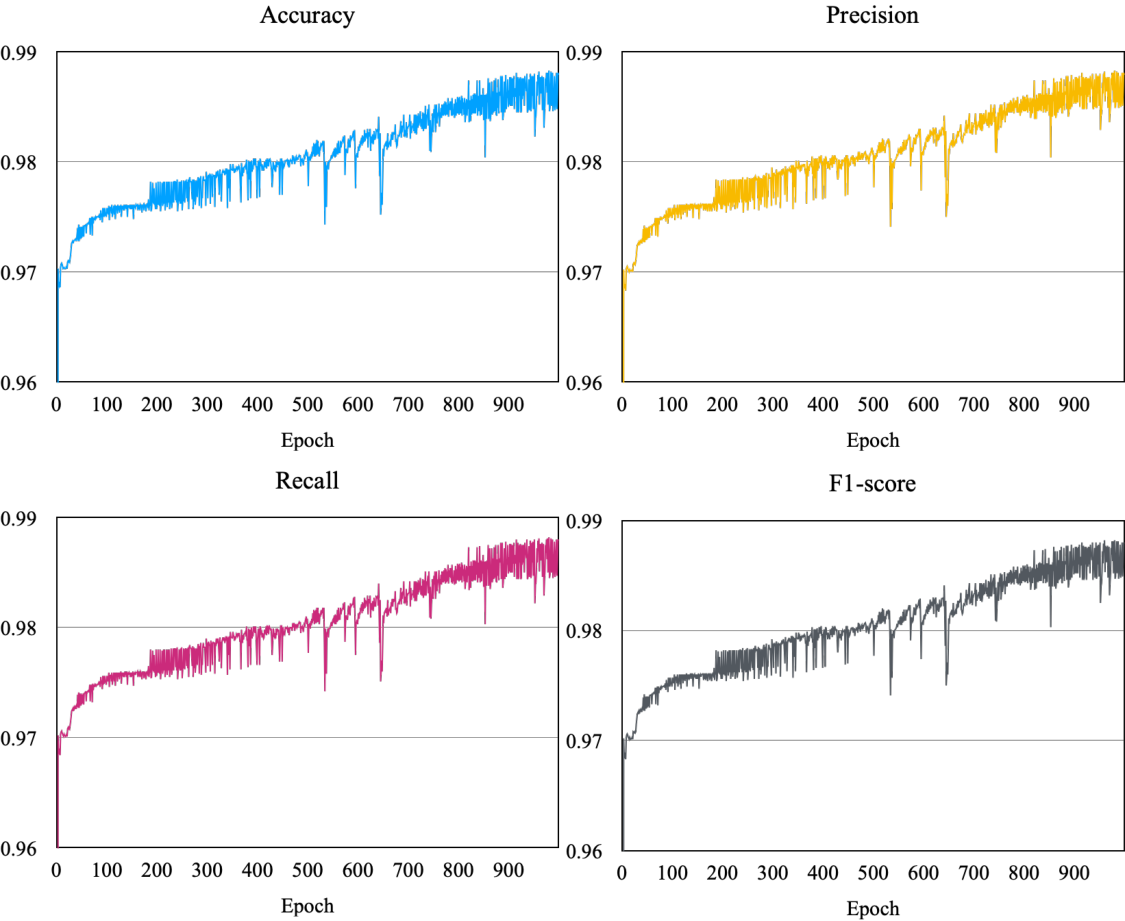
\includegraphics[width = 0.7\linewidth]{Figures/classification effect.pdf}
	\caption{Change curve of classification effect.}
	\label{classification effect}
\end{figure*}



The training employed a data batch size (batch\_size) of 40, the mean squared error loss function (MSELosS), and the Adam gradient optimizer. 
Figure \ref{classification effect} shows the classification effect obtained by testing the entire threat perception model of this paper using the test set after each round of fuser training.
Figure \ref{Loss} illustrates the variation in loss values across different training rounds for the fusion machine based on the fully connected patchwork network.

\begin{figure}[!h]
	\centering
	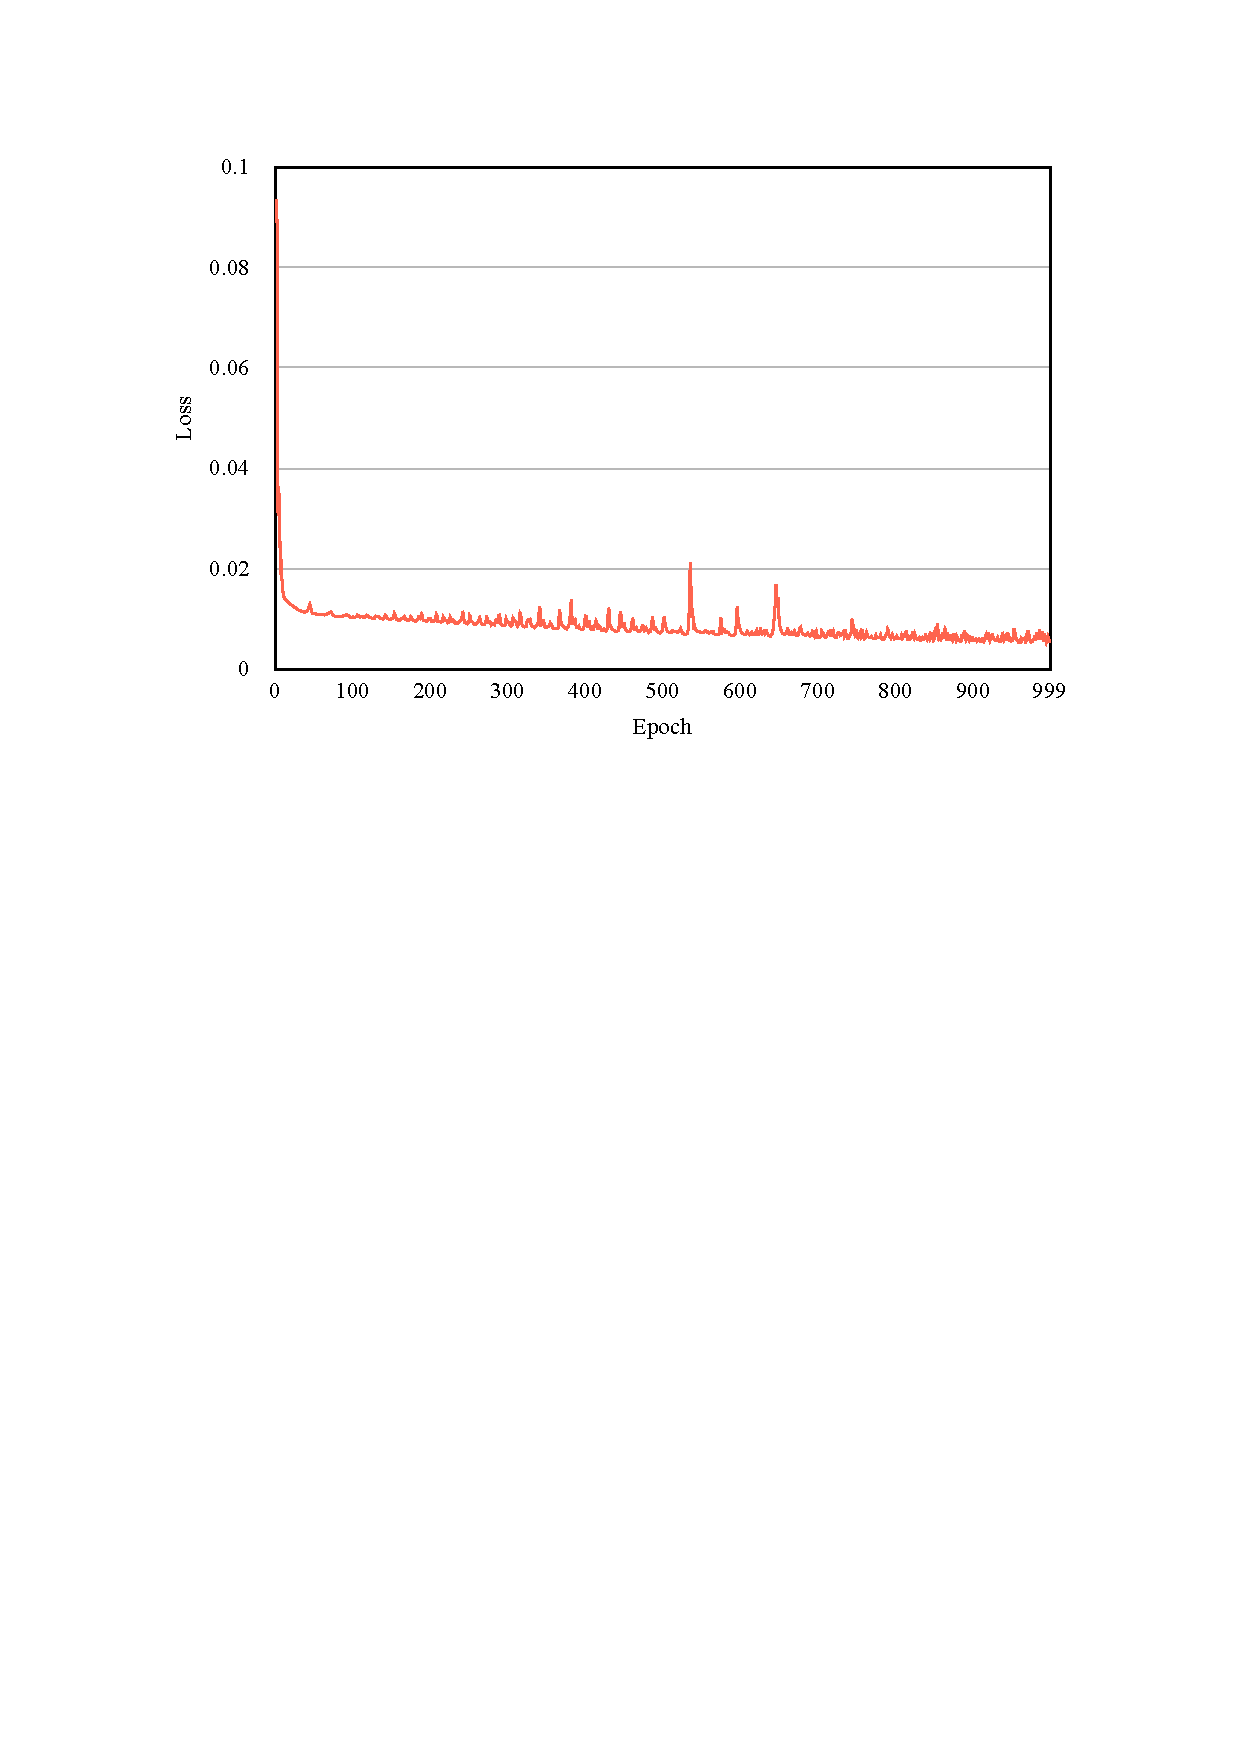
\includegraphics[width = \linewidth]{Figures/Loss.pdf}
	\caption{Loss curve for Fully Connected Neural Networks.}
	\label{Loss}
\end{figure}

As can be seen from the figure, when the number of training rounds is increased from 0 to 800, the accuracy of the threat perception model on the test set as a whole shows a small and slow increase. 
When the number of training rounds is from 800 to 1000, the accuracy rate oscillates around 98\% in a small range and shows a convergence trend.
The curves of Precision, Recall, and F1-score in Figure \ref{classification effect} follow roughly the same trend as the Accuracy curve. 
The classification accuracies can all reach more than 98\% after completing 1000 rounds of fuser training.
It shows that the classification effect can be effectively improved by using the fuser based on a fully connected neural network.
Figure \ref{Loss} reveals that as the number of training rounds increased, the loss value of the fusion machine on the training set decreased, indicating a trend toward convergence. 
This demonstrates that the fusion model progressively improves its classification effectiveness on the test set as training proceeds.

\textbf{Summary:}
After conducting experimental analyses, it is evident that for the multi-classification task scenario of IoT botnet lifecycle detection, the detection result fusion layer, employing a fully connected neural network, can significantly enhance the accuracy of detection results.
It elevates the accuracy from 96.5\% to 98.5\%.
This underscores the necessity and significance of incorporating a detection result fusion layer based on fully connected neural networks.

\textbf{Result 4: Performance of IoT Botnet Lifecycle Detection (Answering Q4)}

To address Q4, we utilized a simulated experimental platform to deploy both botnets and benign services, injecting traffic data into the trained classification model. 
The classification task includes four categories: benign traffic, scanning phase traffic, propagation phase traffic, and attack phase traffic.

To ensure consistency in the number of input features for comparing experimental classifiers (KNN, SVM, LSTM, and our method), we used the complete set of the top 20 important features (comprising 43 different features) obtained from Figure \ref{Important_characteristics} as the feature input for the classification model.

The specific experimental results are detailed in Figure \ref{Confusion_matrix} and Table \ref{Comparison}.

\begin{figure}[!h]
	\centering
	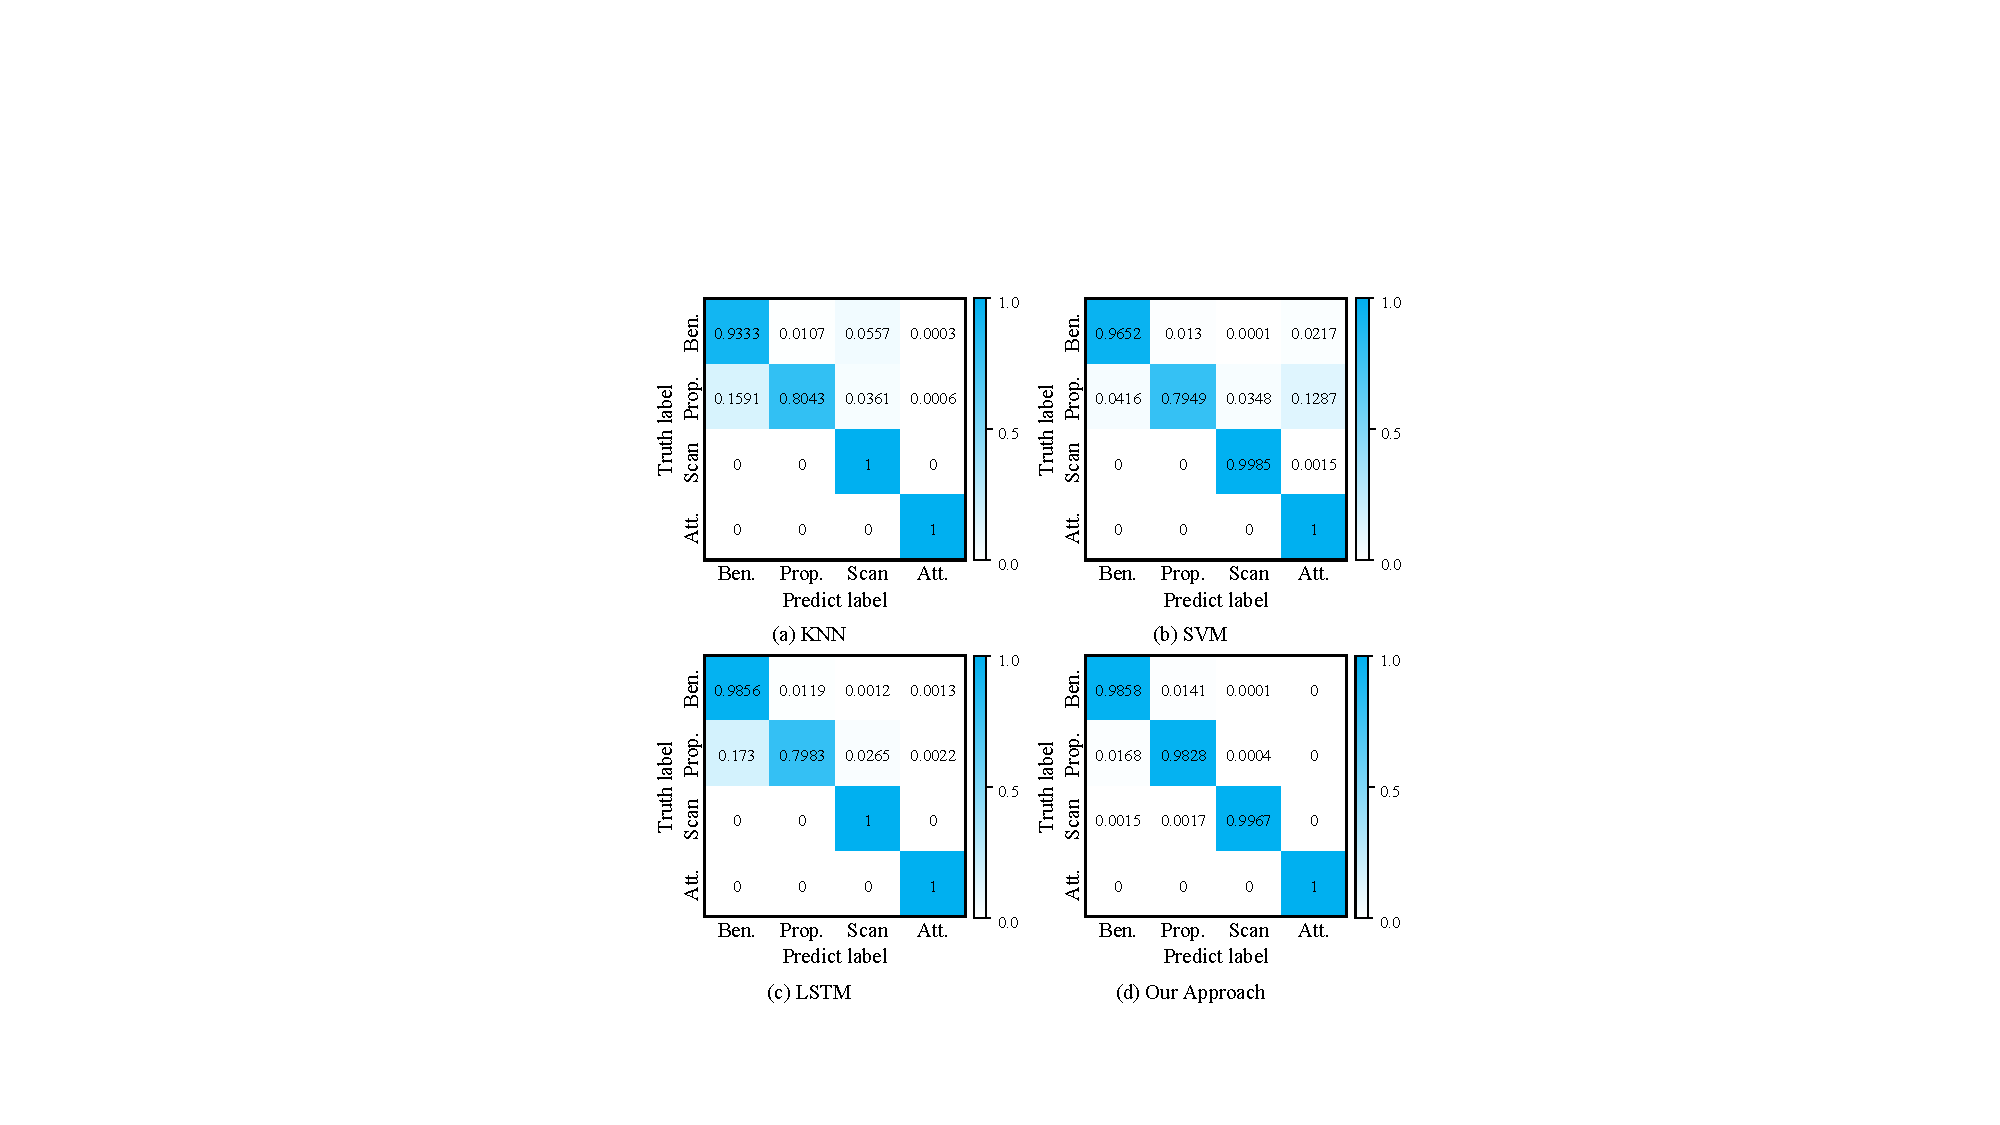
\includegraphics[width = \linewidth]{Figures/confusion matrix.pdf}
	\caption{Confusion matrix for each classifier.}
	\label{Confusion_matrix}
\end{figure}

\begin{table}[!h]
\centering
\caption{Comparison of Classification Effectiveness of Classifiers.}
\label{Comparison}
\begin{tabular}{|c|c|c|c|c|c|}
\hline
Models     & Acc.   & Pre.   & Recall & F1     & Time(ms) \\ \hline
KNN        & 0.9159 & 0.9280 & 0.9159 & 0.9219 & 53240    \\ \hline
SVM        & 0.9289 & 0.9386 & 0.9298 & 0.9342 & 13429    \\ \hline
LSTM       & 0.9412 & 0.9435 & 0.9412 & 0.9423 & 618      \\ \hline
Our method & 0.9881 & 0.9881 & 0.9881 & 0.9881 & 717      \\ \hline
\end{tabular}
\end{table}

Figure \ref{Confusion_matrix} effectively illustrates the classification performance of the four classification models on the test set through a confusion matrix. 
Notably, our approach achieves the highest classification accuracy, surpassing 98\%, when classifying traffic in the propagation phase. 
In contrast, the other three classification models exhibit a classification accuracy of approximately 80%.
Further insights from the confusion matrix reveal that KNN and LSTM misclassify approximately 15.9\% and 17.3\% of propagation stage traffic as benign traffic, respectively. 
In contrast, SVM misclassifies about 12.9\% of propagation phase traffic as attack traffic.
In the classification of benign traffic, our method demonstrates a superior accuracy, with only about 1.4\% of benign traffic being misclassified as malicious traffic.
This result is slightly more accurate than LSTM and SVM, and approximately 5\% more accurate than KNN, which misclassifies more benign traffic (approximately 6.5\%) as scanning phase traffic.

Table \ref{Comparison} provides a clear comparison of the classification performance of the four models, highlighting the advantages of our model over KNN, SVM, and LSTM. 
Notably, our model exhibits improvements in accuracy and other classification metrics. Compared to KNN, it achieves a remarkable 7\% improvement in accuracy. Additionally, when compared to the LSTM classifier, our model demonstrates a substantial 4.5\% enhancement in classification effectiveness metrics such as accuracy.

In terms of classification efficiency, KNN stands out with a test time of 53.24 seconds on the test set, significantly outperforming the other classifiers in the table. This efficiency is attributed to the computational intensity of calculating distances between input samples and the training set during classification. In contrast, our model is 66 times more efficient (time-consuming) than KNN in classification and approximately 16 times better than SVM. These efficiency gains underscore the practical advantages of our model for real-time classification tasks.




\textbf{Summary:}
In comparison to traditional classification models like KNN, SVM, and LSTM, our model stands out in multiple aspects. Notably, it demonstrates:
Enhanced Detection Speed: Our model excels in terms of timely threat detection, significantly outpacing KNN and SVM.

Superior Accuracy: When it comes to classification precision, our model outperforms KNN, SVM, and LSTM.
Reduced False Alarm Rates: We have achieved a notably lower rate of false alarms, which bolsters the model's ability to accurately identify threats while minimizing false positives.

These results underscore the effectiveness and efficiency of our model for IoT botnet lifecycle detection, positioning it as a valuable asset in the realm of cybersecurity.






\section{Conclusion}
In this research paper, we present RGPot, a generative response honeypot designed for IoT botnet lifecycle detection.
RGPot consists of two basic components: an interaction response module and a lifecycle detection module.
The interaction response module uses a generative adversarial network model to generate appropriate response data for various IoT protocol request data.
This adaptability enables RGPot to respond effectively to different IoT communication protocols in complex IoT environments.
On the other hand, the lifecycle detection module employs long and short-term memory network model fusion techniques to accurately identify the lifecycle phases of IoT botnet traffic.
It can distinguish whether the interactive traffic is malicious or not, and if it is, it can also pinpoint the specific phase of the botnet life cycle.
We demonstrate the efficacy of RGPot through simulations and comparative experiments.
It generates response data that closely resembles real data, demonstrating its ability to proficiently interact with IoT botnets.
In addition, RGPot demonstrated high accuracy and low false alarm rate in IoT botnet lifecycle detection.

Going forward, our work will include incorporating more diverse IoT data to further enhance RGPot's training.
In addition, we plan to deploy RGPot in public network environments to extend its ability to accurately identify a wider range of IoT botnet traffic data.



%% The Appendices part is started with the command \appendix;
%% appendix sections are then done as normal sections
%% \appendix


%% The Appendices part is started with the command \appendix;
%% appendix sections are then done as normal sections
%% \appendix

%% \section{}
%% \label{}

%% If you have bibdatabase file and want bibtex to generate the
%% bibitems, please use
%%







\bibliographystyle{IEEEtran}
\bibliography{references}



\end{document}
